% answers.tex —— 2012 年·山东卷·理科 · 参考答案与详细解析片段
% 由 tools/generate_projects.py 依来源总账自 2012/2012_数学真题_山东理_试题.md + 2012/2012_数学真题_山东理_解析正文.md + 2012/2012_数学真题_山东理_答案要点.md 生成，勿手改（改源 MD 后重跑）

\begin{answer}
\gksolhead{1}{}

\textbf{题目}：

若复数 $z$ 满足 $z(2-\mathrm i)=11+7\mathrm i$（$\mathrm i$ 为虚数单位），则 $z$ 为\mbox{（　　）}

（A）$3+5\mathrm i$；（B）$3-5\mathrm i$；（C）$-3+5\mathrm i$；（D）$-3-5\mathrm i$。

\Needspace{4\baselineskip}
\textbf{解析}
\nopagebreak[4]
\[z=\frac{11+7\mathrm i}{2-\mathrm i}=\frac{(11+7\mathrm i)(2+\mathrm i)}{5}=\frac{15+25\mathrm i}{5}=3+5\mathrm i.\]
选 A。

\gkanswer{答案：A。}

\end{answer}
\begin{answer}
\gksolhead{2}{}

\textbf{题目}：

已知全集 $U=\{0,1,2,3,4\}$，集合 $A=\{1,2,3\}$，$B=\{2,4\}$，则 $\complement_UA\cup B=$\mbox{（　　）}

（A）$\{1,2,4\}$；（B）$\{2,3,4\}$；（C）$\{0,2,4\}$；（D）$\{0,2,3,4\}$。

\Needspace{4\baselineskip}
\textbf{解析}
$\complement_UA=\{0,4\}$，故 $\complement_UA\cup B=\{0,4\}\cup\{2,4\}=\{0,2,4\}$。选 C。

\gkanswer{答案：C。}

\end{answer}
\begin{answer}
\gksolhead{3}{}

\textbf{题目}：

设 $a>0$ 且 $a\neq1$，则「函数 $f(x)=a^x$ 在 $\mathbf R$ 上是减函数」是「函数 $g(x)=(2-a)x^3$ 在 $\mathbf R$ 上是增函数」的\mbox{（　　）}

（A）充分不必要条件；（B）必要不充分条件；（C）充分必要条件；（D）既不充分也不必要条件。

\Needspace{4\baselineskip}
\textbf{解析}
$f(x)=a^x$ 在 $\mathbf R$ 上递减等价于 $0<a<1$；$g(x)=(2-a)x^3$ 在 $\mathbf R$ 上递增等价于 $2-a>0$，即 $a<2$。由 $0<a<1$ 可推出 $a<2$，反之不成立（如 $a=\dfrac32$）。故为充分不必要条件。选 A。

\gkanswer{答案：A。}

\end{answer}
\begin{answer}
\gksolhead{4}{}

\textbf{题目}：

采用系统抽样方法从 $960$ 人中抽取 $32$ 人做问卷调查。为此将他们随机编号为 $1$, $2$, $\cdots$, $960$，分组后在第一组采用简单随机抽样的方法抽到的号码为 $9$。抽到的 $32$ 人中，编号落入区间 $[1,450]$ 的人做问卷 $A$，编号落入区间 $[451,750]$ 的人做问卷 $B$，其余的人做问卷 $C$。则抽到的人中，做问卷 $B$ 的人数为\mbox{（　　）}

（A）$7$；（B）$9$；（C）$10$；（D）$15$。

\Needspace{4\baselineskip}
\textbf{解析}
\Needspace{5\baselineskip}
抽样间隔为 $\dfrac{960}{32}=30$，抽到的号码为 $9+30k$（$k=0,1,\cdots,31$）。令
\nopagebreak[4]
\[451\leqslant9+30k\leqslant750,\]
得 $14.73\leqslant k\leqslant24.7$，故 $k=15,16,\cdots,24$，共 $10$ 人。选 C。

\gkanswer{答案：C。}

\end{answer}
\begin{answer}
\gksolhead{5}{}

\textbf{题目}：

设变量 $x$，$y$ 满足约束条件 $\begin{cases}x+2y\geqslant2,\\2x+y\leqslant4,\\4x-y\geqslant-1,\end{cases}$ 则目标函数 $z=3x-y$ 的取值范围是\mbox{（　　）}

（A）$\left[-\dfrac32,6\right]$；（B）$\left[-\dfrac32,-1\right]$；（C）$[-1,6]$；（D）$\left[-6,\dfrac32\right]$。

\Needspace{4\baselineskip}
\textbf{解析}
三条边界两两相交得 $(2,0)$，$\left(\dfrac12,3\right)$，$(0,1)$。$z=3x-y$ 在这三点取值 $6$，$-\dfrac32$，$-1$，故取值范围为 $\left[-\dfrac32,6\right]$。选 A。

\gkanswer{答案：A。}

\end{answer}
\begin{answer}
\gksolhead{6}{}

\textbf{题目}：

执行如图所示的程序框图，如果输入 $a=4$，那么输出的 $n$ 的值为\mbox{（　　）}
\nopagebreak[4]
\begin{center}%% ============================================================
% f2012_shandong_sci_q06_flowchart.tex
%% 2012 山东卷（理科）第 6 题 程序框图
%% 来源 PDF：普通高考/2012/2012山东理.pdf 第 1 页（印面 759）第 1 栏
%% 坐标取自原页矢量层（bp），原点为图区左上角 (145.0,548.0)，y 向下。
%% 流程：开始 → 输入 a → P=0,Q=1,n=0 → 判断 P⩽Q
%%   是 → P=P+a^n → Q=2Q+1 → n=n+1 → 回判断；否 → 输出 n → 结束
%% ============================================================
\begin{tikzpicture}[x=1bp,y=-1bp,
  every node/.style={inner sep=0,font=\fontsize{10.5pt}{12.6pt}\selectfont},
  line cap=butt, line join=miter]
  \draw[line width=0.398bp] (67.805,7.723) -- (47.781,7.723) .. controls (45.582,7.723) and (43.797,9.508) .. (43.797,11.707) -- (43.797,20.57) .. controls (43.797,22.773) and (45.582,24.555) .. (47.781,24.555) -- (67.805,24.555) .. controls (70.004,24.555) and (71.785,22.773) .. (71.785,20.57) -- (71.785,11.707) .. controls (71.785,9.508) and (70.004,7.723) .. (67.805,7.723) -- cycle;
  \draw[line width=0.398bp] (33.148,55.957) -- (39.273,39.125) -- (82.43,39.125) -- (76.305,55.957) -- cycle;
  \draw[line width=0.398bp] (7.621,86.734) -- (107.965,86.734) -- (107.965,70.523) -- (7.621,70.523) -- cycle;
  \draw[line width=0.398bp] (98.852,111.586) -- (57.793,101.383) -- (16.734,111.586) -- (57.793,121.789) -- cycle;
  \draw[line width=0.398bp] (27.199,151.48) -- (88.383,151.48) -- (88.383,136.437) -- (27.199,136.437) -- cycle;
  \draw[line width=0.398bp] (27.336,182.258) -- (88.25,182.258) -- (88.25,166.047) -- (27.336,166.047) -- cycle;
  \draw[line width=0.398bp] (31.957,211.461) -- (83.625,211.461) -- (83.625,196.824) -- (31.957,196.824) -- cycle;
  \draw[line width=0.398bp] (99.895,152.387) -- (106.031,135.531) -- (149.945,135.531) -- (143.812,152.387) -- cycle;
  \draw[line width=0.398bp] (134.934,166.953) -- (114.914,166.953) .. controls (112.715,166.953) and (110.93,168.734) .. (110.93,170.937) -- (110.93,179.98) .. controls (110.93,182.18) and (112.715,183.961) .. (114.914,183.961) -- (134.934,183.961) .. controls (137.137,183.961) and (138.918,182.18) .. (138.918,179.98) -- (138.918,170.937) .. controls (138.918,168.734) and (137.137,166.953) .. (134.934,166.953) -- cycle;
  \draw[line width=0.398bp] (57.793,24.754) -- (57.793,35.336);
  \fill[black] (57.793,38.922) .. controls (57.992,37.859) and (58.59,36.133) .. (59.285,34.938) -- (56.301,34.938) .. controls (56.996,36.133) and (57.594,37.859) .. (57.793,38.922);
  \draw[line width=0.398bp] (57.793,56.156) -- (57.793,66.738);
  \fill[black] (57.793,70.324) .. controls (57.992,69.262) and (58.59,67.535) .. (59.285,66.34) -- (56.297,66.34) .. controls (56.996,67.535) and (57.594,69.262) .. (57.793,70.324);
  \draw[line width=0.398bp] (57.793,86.934) -- (57.793,97.516);
  \fill[black] (57.793,101.102) .. controls (57.992,100.039) and (58.59,98.312) .. (59.285,97.117) -- (56.301,97.117) .. controls (56.996,98.312) and (57.594,100.039) .. (57.793,101.102);
  \draw[line width=0.398bp] (57.793,122.07) -- (57.793,132.652);
  \fill[black] (57.793,136.238) .. controls (57.992,135.176) and (58.59,133.449) .. (59.285,132.254) -- (56.301,132.254) .. controls (56.996,133.449) and (57.594,135.176) .. (57.793,136.238);
  \draw[line width=0.398bp] (57.793,151.68) -- (57.793,162.262);
  \fill[black] (57.793,165.848) .. controls (57.992,164.785) and (58.59,163.059) .. (59.285,161.863) -- (56.301,161.863) .. controls (56.996,163.059) and (57.594,164.785) .. (57.793,165.848);
  \draw[line width=0.398bp] (57.793,182.457) -- (57.793,193.039);
  \fill[black] (57.793,196.625) .. controls (57.992,195.562) and (58.59,193.836) .. (59.285,192.641) -- (56.301,192.641) .. controls (56.996,193.836) and (57.594,195.562) .. (57.793,196.625);
  \draw[line width=0.398bp] (124.926,152.586) -- (124.922,163.168);
  \fill[black] (124.922,166.754) .. controls (125.121,165.691) and (125.719,163.965) .. (126.418,162.77) -- (123.43,162.77) .. controls (124.129,163.965) and (124.727,165.691) .. (124.922,166.754);
  \draw[line width=0.398bp] (57.793,211.656) -- (57.793,217.324) -- (6.789,217.324) -- (6.789,94.016) -- (54.207,94.016);
  \fill[black] (57.793,94.016) .. controls (56.73,93.816) and (55.004,93.219) .. (53.809,92.523) -- (53.809,95.512) .. controls (55.004,94.812) and (56.73,94.215) .. (57.793,94.016);
  \draw[line width=0.398bp] (99.133,111.586) -- (124.926,111.586) -- (124.926,131.746);
  \fill[black] (124.926,135.332) .. controls (125.125,134.27) and (125.723,132.543) .. (126.418,131.348) -- (123.43,131.348) .. controls (124.129,132.543) and (124.727,134.27) .. (124.926,135.332);
  \node[anchor=base west] at (47.37,20.92) {$\text{开始}$};
  \node[anchor=base west] at (42.84,52.29) {$\text{输入}\ a$};
  \node[anchor=base west] at (11.18,83.37) {$P=0,\ Q=1,\ n=0$};
  \node[anchor=base west] at (42.62,116.33) {$P\leqslant Q$};
  \node[anchor=base west] at (61.57,133.87) {$\text{是}$};
  \node[anchor=base west] at (93.97,108.01) {$\text{否}$};
  \node[anchor=base west] at (30.77,149.3) {$P=P+a^n$};
  \node[anchor=base west] at (30.9,178.92) {$Q=2Q+1$};
  \node[anchor=base west] at (35.53,209.3) {$n=n+1$};
  \node[anchor=base west] at (109.62,148.75) {$\text{输出}\ n$};
  \node[anchor=base west] at (114.53,180.27) {$\text{结束}$};
\end{tikzpicture}
\end{center}
\nopagebreak[4]
（A）$2$；（B）$3$；（C）$4$；（D）$5$。

\Needspace{4\baselineskip}
\textbf{解析}
\Needspace{5\baselineskip}
初始 $P=0$，$Q=1$，$n=0$。当 $P\leqslant Q$ 时执行 $P=P+4^n$，$Q=2Q+1$，$n=n+1$：
\nopagebreak[4]
\[(P,Q,n)=(1,3,1)\to(5,7,2)\to(21,15,3).\]
此时 $21\leqslant15$ 不成立，输出 $n=3$。选 B。

\gkanswer{答案：B。}

\end{answer}
\begin{answer}
\gksolhead{7}{}

\textbf{题目}：

若 $\theta\in\left[\dfrac\pi4,\dfrac\pi2\right]$，$\sin2\theta=\dfrac{3\sqrt7}8$，则 $\sin\theta=$\mbox{（　　）}

（A）$\dfrac35$；（B）$\dfrac45$；（C）$\dfrac{\sqrt7}4$；（D）$\dfrac34$。

\Needspace{4\baselineskip}
\textbf{解析}
\Needspace{5\baselineskip}
由 $\theta\in\left[\dfrac\pi4,\dfrac\pi2\right]$ 得 $2\theta\in\left[\dfrac\pi2,\pi\right]$，故 $\cos2\theta<0$，
\nopagebreak[4]
\[\cos2\theta=-\sqrt{1-\sin^22\theta}=-\sqrt{1-\frac{63}{64}}=-\frac18.\]
\Needspace{5\baselineskip}
于是
\nopagebreak[4]
\[\sin\theta=\sqrt{\frac{1-\cos2\theta}2}=\sqrt{\frac{9}{16}}=\frac34.\]
选 D。

\gkanswer{答案：D。}

\end{answer}
\begin{answer}
\gksolhead{8}{}

\textbf{题目}：

定义在 $\mathbf R$ 上的函数 $f(x)$ 满足 $f(x+6)=f(x)$。当 $-3\leqslant x<-1$ 时，$f(x)=-(x+2)^2$；当 $-1\leqslant x<3$ 时，$f(x)=x$。则 $f(1)+f(2)+\cdots+f(2012)=$\mbox{（　　）}

（A）$335$；（B）$338$；（C）$1678$；（D）$2012$。

\Needspace{4\baselineskip}
\textbf{解析}
\Needspace{5\baselineskip}
由 $f(x+6)=f(x)$ 知 $f$ 以 $6$ 为周期。在一个周期内
\nopagebreak[4]
\[f(1)=1,\quad f(2)=2,\quad f(3)=f(-3)=-1,\]
\nopagebreak[4]
\[f(4)=f(-2)=0,\quad f(5)=f(-1)=-1,\quad f(6)=f(0)=0,\]
\Needspace{5\baselineskip}
其和为 $1$。由 $2012=6\times335+2$ 得
\nopagebreak[4]
\[\sum_{k=1}^{2012}f(k)=335\times1+f(2011)+f(2012)=335+1+2=338.\]
选 B。

\gkanswer{答案：B。}

\end{answer}
\begin{answer}
\gksolhead{9}{}

\textbf{题目}：

函数 $f(x)=\dfrac{\cos6x}{2^x-2^{-x}}$ 的图象大致为\mbox{（　　）}
\nopagebreak[4]
\begin{center}%% ============================================================
%% f2012_shandong_sci_q09_graphs.tex
%% 2012 山东卷（理科）第 9 题 四个选项的函数图象（选项图）
%% 来源 PDF：普通高考/2012/2012山东理.pdf 第 1 页（印面 759）第 2 栏
%% 坐标取自原页矢量层（bp），原点为图区左上角 (458.0,207.0)，y 向下；
%% 坐标轴、箭头与曲线均为原页路径逐条复刻（曲线为原页折线路径，未重新拟合）。
%% 题干函数 f(x)=cos6x/(2^x-2^-x)：y 轴右侧紧邻处 f→+∞（在 x 轴上方），左侧紧邻处 f→-∞；
%% 与原页矢量路径的归一化最小二乘比对：仅 (D) 与该函数族一致（rms/amp=0.0029），
%% (B) 恰为 -f（左右符号相反），(A)(C) 不能用该族拟合（rms/amp≥0.28）。故答案 D。
%% ============================================================
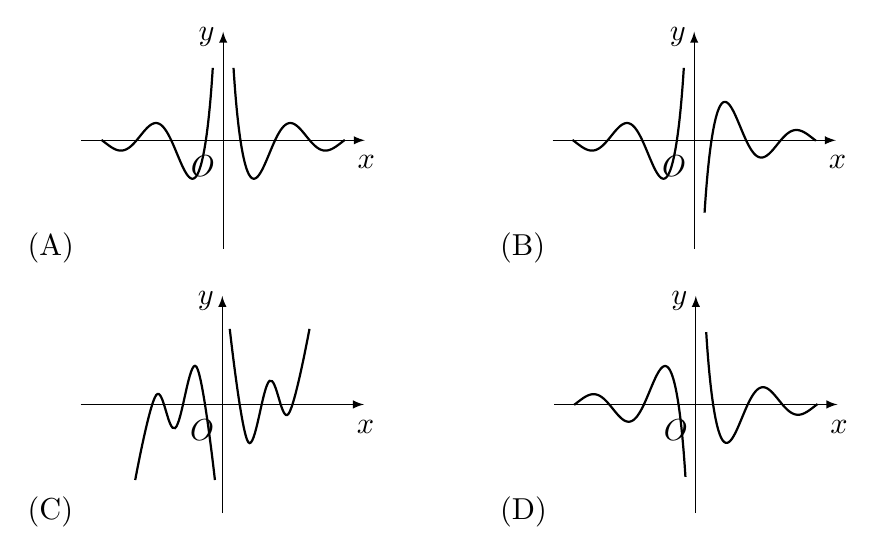
\begin{tikzpicture}[x=1bp,y=-1bp,
  every node/.style={inner sep=0,font=\fontsize{10.5pt}{12.6pt}\selectfont},
  line cap=butt, line join=miter]
  \draw[line width=0.398bp] (0.816,58.395) -- (99.242,58.395);
  \fill[black] (102.828,58.395) .. controls (101.766,58.195) and (100.039,57.598) .. (98.844,56.902) -- (98.844,59.887) .. controls (100.039,59.191) and (101.766,58.594) .. (102.828,58.395);
  \draw[line width=0.398bp] (51.824,97.5) -- (51.824,22.875);
  \fill[black] (51.824,19.289) .. controls (51.625,20.352) and (51.027,22.078) .. (50.328,23.273) -- (53.316,23.273) .. controls (52.617,22.078) and (52.02,20.352) .. (51.824,19.289);
  \draw[line width=0.797bp] (55.559,32.332) -- (55.691,34.41) -- (55.828,36.387) -- (55.961,38.266) -- (56.094,40.039) -- (56.23,41.73) -- (56.363,43.336) -- (56.496,44.863) -- (56.633,46.324) -- (56.766,47.723) -- (56.898,49.055) -- (57.035,50.328) -- (57.168,51.547) -- (57.301,52.711) -- (57.434,53.828) -- (57.57,54.895) -- (57.703,55.922) -- (57.836,56.902) -- (57.973,57.84) -- (58.105,58.738) -- (58.238,59.598) -- (58.375,60.422) -- (58.508,61.211) -- (58.641,61.961) -- (58.777,62.684) -- (58.91,63.371) -- (59.043,64.023) -- (59.176,64.648) -- (59.312,65.246) -- (59.445,65.812) -- (59.578,66.352) -- (59.715,66.859) -- (59.848,67.344) -- (59.98,67.801) -- (60.117,68.234) -- (60.25,68.637) -- (60.383,69.02) -- (60.52,69.379) -- (60.652,69.711) -- (60.785,70.023) -- (60.922,70.312) -- (61.055,70.578) -- (61.187,70.82) -- (61.32,71.047) -- (61.457,71.246) -- (61.59,71.43) -- (61.723,71.594) -- (61.859,71.734) -- (61.992,71.855) -- (62.125,71.961) -- (62.262,72.047) -- (62.395,72.117) -- (62.527,72.168) -- (62.664,72.203) -- (62.797,72.219) -- (62.93,72.223) -- (63.062,72.207) -- (63.199,72.18) -- (63.332,72.133) -- (63.465,72.074) -- (63.602,72) -- (63.734,71.91) -- (63.867,71.809) -- (64.004,71.695) -- (64.137,71.57) -- (64.27,71.43) -- (64.406,71.281) -- (64.539,71.117) -- (64.672,70.945) -- (64.805,70.762) -- (64.941,70.566) -- (65.074,70.363) -- (65.207,70.148) -- (65.344,69.926) -- (65.477,69.695) -- (65.609,69.457) -- (65.746,69.211) -- (65.879,68.957) -- (66.012,68.695) -- (66.145,68.426) -- (66.281,68.152) -- (66.414,67.871) -- (66.551,67.586) -- (66.684,67.297) -- (66.816,67.004) -- (66.949,66.699) -- (67.086,66.398) -- (67.352,65.781) -- (67.488,65.469) -- (67.754,64.836) -- (67.887,64.516) -- (68.023,64.195) -- (68.156,63.875) -- (68.293,63.551) -- (68.426,63.227) -- (68.559,62.906) -- (68.691,62.582) -- (68.828,62.262) -- (68.961,61.941) -- (69.094,61.625) -- (69.23,61.305) -- (69.363,60.988) -- (69.496,60.676) -- (69.629,60.367) -- (69.766,60.059) -- (69.898,59.754) -- (70.035,59.449) -- (70.301,58.855) -- (70.434,58.566) -- (70.57,58.281) -- (70.703,58.004) -- (70.836,57.723) -- (70.973,57.453) -- (71.105,57.187) -- (71.238,56.93) -- (71.375,56.672) -- (71.508,56.422) -- (71.641,56.18) -- (71.773,55.941) -- (71.91,55.711) -- (72.043,55.488) -- (72.18,55.27) -- (72.312,55.059) -- (72.445,54.855) -- (72.578,54.656) -- (72.715,54.469) -- (72.848,54.285) -- (72.98,54.109) -- (73.117,53.941) -- (73.25,53.781) -- (73.383,53.629) -- (73.516,53.48) -- (73.652,53.344) -- (73.785,53.215) -- (73.922,53.094) -- (74.055,52.977) -- (74.187,52.871) -- (74.32,52.773) -- (74.457,52.68) -- (74.59,52.598) -- (74.723,52.52) -- (74.859,52.453) -- (74.992,52.395) -- (75.125,52.344) -- (75.258,52.297) -- (75.395,52.262) -- (75.527,52.23) -- (75.664,52.207) -- (75.797,52.191) -- (76.062,52.184) -- (76.199,52.191) -- (76.332,52.207) -- (76.465,52.227) -- (76.602,52.254) -- (76.734,52.289) -- (76.867,52.328) -- (77.004,52.375) -- (77.137,52.434) -- (77.27,52.488) -- (77.402,52.559) -- (77.539,52.629) -- (77.672,52.707) -- (77.809,52.793) -- (77.941,52.879) -- (78.074,52.973) -- (78.207,53.07) -- (78.344,53.176) -- (78.609,53.395) -- (78.746,53.516) -- (78.879,53.637) -- (79.012,53.762) -- (79.145,53.895) -- (79.281,54.023) -- (79.414,54.164) -- (79.551,54.305) -- (79.684,54.445) -- (79.949,54.742) -- (80.086,54.895) -- (80.219,55.047) -- (80.352,55.203) -- (80.488,55.359) -- (80.887,55.84) -- (81.023,56.008) -- (81.156,56.172) -- (81.293,56.336) -- (81.559,56.664) -- (81.691,56.832) -- (81.828,56.996) -- (81.961,57.164) -- (82.094,57.328) -- (82.23,57.492) -- (82.496,57.82) -- (82.629,57.98) -- (82.766,58.145) -- (82.898,58.301) -- (83.035,58.457) -- (83.168,58.613) -- (83.301,58.766) -- (83.437,58.918) -- (83.703,59.215) -- (83.836,59.359) -- (83.973,59.5) -- (84.105,59.641) -- (84.238,59.777) -- (84.375,59.91) -- (84.641,60.168) -- (84.773,60.289) -- (84.91,60.41) -- (85.043,60.527) -- (85.176,60.641) -- (85.312,60.75) -- (85.445,60.855) -- (85.578,60.957) -- (85.715,61.055) -- (85.98,61.234) -- (86.117,61.32) -- (86.25,61.402) -- (86.516,61.551) -- (86.652,61.617) -- (86.785,61.68) -- (86.918,61.738) -- (87.055,61.793) -- (87.187,61.844) -- (87.32,61.891) -- (87.457,61.93) -- (87.59,61.969) -- (87.723,62) -- (87.859,62.027) -- (87.992,62.051) -- (88.125,62.07) -- (88.258,62.082) -- (88.395,62.094) -- (88.66,62.102) -- (88.797,62.098) -- (88.93,62.09) -- (89.062,62.078) -- (89.199,62.062) -- (89.332,62.043) -- (89.465,62.02) -- (89.602,61.992) -- (89.734,61.961) -- (89.867,61.926) -- (90.004,61.887) -- (90.137,61.844) -- (90.402,61.75) -- (90.539,61.695) -- (90.672,61.641) -- (90.805,61.582) -- (90.941,61.516) -- (91.207,61.383) -- (91.344,61.312) -- (91.477,61.238) -- (91.609,61.16) -- (91.746,61.082) -- (92.012,60.918) -- (92.145,60.832) -- (92.281,60.742) -- (92.414,60.656) -- (92.547,60.562) -- (92.684,60.469) -- (92.949,60.281) -- (93.086,60.184) -- (93.219,60.086) -- (93.352,59.984) -- (93.488,59.883) -- (93.621,59.785) -- (93.754,59.684) -- (93.887,59.578) -- (94.023,59.477) -- (94.156,59.375) -- (94.289,59.27) -- (94.426,59.168) -- (94.559,59.066) -- (94.691,58.961) -- (94.828,58.859) -- (95.094,58.656) -- (95.23,58.555) -- (95.363,58.453) -- (95.496,58.355) -- (95.633,58.254);
  \draw[line width=0.797bp] (48.086,32.332) -- (47.953,34.41) -- (47.816,36.387) -- (47.684,38.266) -- (47.551,40.039) -- (47.414,41.73) -- (47.281,43.336) -- (47.148,44.863) -- (47.012,46.324) -- (46.879,47.723) -- (46.746,49.055) -- (46.609,50.328) -- (46.477,51.547) -- (46.344,52.711) -- (46.211,53.828) -- (46.074,54.895) -- (45.941,55.922) -- (45.809,56.902) -- (45.672,57.84) -- (45.539,58.738) -- (45.406,59.598) -- (45.27,60.422) -- (45.137,61.211) -- (45.004,61.961) -- (44.867,62.684) -- (44.734,63.371) -- (44.602,64.023) -- (44.469,64.648) -- (44.332,65.246) -- (44.199,65.812) -- (44.066,66.352) -- (43.93,66.859) -- (43.797,67.344) -- (43.664,67.801) -- (43.527,68.234) -- (43.395,68.637) -- (43.262,69.02) -- (43.125,69.379) -- (42.992,69.711) -- (42.859,70.023) -- (42.723,70.312) -- (42.59,70.578) -- (42.457,70.82) -- (42.324,71.047) -- (42.188,71.246) -- (42.055,71.43) -- (41.922,71.594) -- (41.785,71.734) -- (41.652,71.855) -- (41.52,71.961) -- (41.383,72.047) -- (41.25,72.117) -- (41.117,72.168) -- (40.98,72.203) -- (40.848,72.219) -- (40.715,72.223) -- (40.582,72.207) -- (40.445,72.18) -- (40.313,72.133) -- (40.18,72.074) -- (40.043,72) -- (39.91,71.91) -- (39.777,71.809) -- (39.641,71.695) -- (39.508,71.57) -- (39.375,71.43) -- (39.238,71.281) -- (39.105,71.117) -- (38.973,70.945) -- (38.84,70.762) -- (38.703,70.566) -- (38.57,70.363) -- (38.438,70.148) -- (38.301,69.926) -- (38.168,69.695) -- (38.035,69.457) -- (37.898,69.211) -- (37.766,68.957) -- (37.633,68.695) -- (37.5,68.426) -- (37.363,68.152) -- (37.23,67.871) -- (37.094,67.586) -- (36.961,67.297) -- (36.828,67.004) -- (36.695,66.699) -- (36.559,66.398) -- (36.293,65.781) -- (36.156,65.469) -- (35.891,64.836) -- (35.758,64.516) -- (35.621,64.195) -- (35.488,63.875) -- (35.352,63.551) -- (35.219,63.227) -- (35.086,62.906) -- (34.953,62.582) -- (34.816,62.262) -- (34.684,61.941) -- (34.551,61.625) -- (34.414,61.305) -- (34.281,60.988) -- (34.148,60.676) -- (34.016,60.367) -- (33.879,60.059) -- (33.746,59.754) -- (33.609,59.449) -- (33.344,58.855) -- (33.211,58.566) -- (33.074,58.281) -- (32.941,58.004) -- (32.809,57.723) -- (32.672,57.453) -- (32.539,57.187) -- (32.273,56.672) -- (32.137,56.422) -- (32.004,56.18) -- (31.871,55.941) -- (31.734,55.711) -- (31.602,55.488) -- (31.465,55.27) -- (31.332,55.059) -- (31.199,54.855) -- (31.066,54.656) -- (30.93,54.469) -- (30.797,54.285) -- (30.664,54.109) -- (30.527,53.941) -- (30.395,53.781) -- (30.262,53.629) -- (30.129,53.48) -- (29.992,53.344) -- (29.859,53.215) -- (29.723,53.094) -- (29.59,52.977) -- (29.457,52.871) -- (29.324,52.773) -- (29.188,52.68) -- (29.055,52.598) -- (28.922,52.52) -- (28.785,52.453) -- (28.652,52.395) -- (28.52,52.344) -- (28.387,52.297) -- (28.25,52.262) -- (28.117,52.23) -- (27.98,52.207) -- (27.848,52.191) -- (27.582,52.184) -- (27.445,52.191) -- (27.313,52.207) -- (27.18,52.227) -- (27.043,52.254) -- (26.91,52.289) -- (26.777,52.328) -- (26.645,52.375) -- (26.508,52.434) -- (26.375,52.488) -- (26.242,52.559) -- (26.105,52.629) -- (25.973,52.707) -- (25.84,52.793) -- (25.703,52.879) -- (25.57,52.973) -- (25.438,53.07) -- (25.301,53.176) -- (25.035,53.395) -- (24.898,53.516) -- (24.766,53.637) -- (24.633,53.762) -- (24.5,53.895) -- (24.363,54.023) -- (24.23,54.164) -- (24.094,54.305) -- (23.961,54.445) -- (23.695,54.742) -- (23.559,54.895) -- (23.426,55.047) -- (23.293,55.203) -- (23.156,55.359) -- (22.758,55.84) -- (22.621,56.008) -- (22.488,56.172) -- (22.352,56.336) -- (22.086,56.664) -- (21.953,56.832) -- (21.816,56.996) -- (21.684,57.164) -- (21.551,57.328) -- (21.414,57.492) -- (21.148,57.82) -- (21.016,57.98) -- (20.879,58.145) -- (20.746,58.301) -- (20.609,58.457) -- (20.477,58.613) -- (20.211,58.918) -- (20.074,59.066) -- (19.941,59.215) -- (19.809,59.359) -- (19.672,59.5) -- (19.539,59.641) -- (19.406,59.777) -- (19.27,59.91) -- (19.004,60.168) -- (18.871,60.289) -- (18.734,60.41) -- (18.602,60.527) -- (18.469,60.641) -- (18.332,60.75) -- (18.199,60.855) -- (18.066,60.957) -- (17.93,61.055) -- (17.664,61.234) -- (17.527,61.32) -- (17.395,61.402) -- (17.129,61.551) -- (16.992,61.617) -- (16.859,61.68) -- (16.727,61.738) -- (16.59,61.793) -- (16.457,61.844) -- (16.324,61.891) -- (16.188,61.93) -- (16.055,61.969) -- (15.922,62) -- (15.785,62.027) -- (15.652,62.051) -- (15.52,62.07) -- (15.387,62.082) -- (15.25,62.094) -- (14.984,62.102) -- (14.848,62.098) -- (14.715,62.09) -- (14.582,62.078) -- (14.445,62.062) -- (14.313,62.043) -- (14.18,62.02) -- (14.043,61.992) -- (13.91,61.961) -- (13.777,61.926) -- (13.641,61.887) -- (13.508,61.844) -- (13.242,61.75) -- (13.105,61.695) -- (12.973,61.641) -- (12.84,61.582) -- (12.703,61.516) -- (12.438,61.383) -- (12.301,61.312) -- (12.168,61.238) -- (12.035,61.16) -- (11.898,61.082) -- (11.633,60.918) -- (11.5,60.832) -- (11.363,60.742) -- (11.23,60.656) -- (11.098,60.562) -- (10.961,60.469) -- (10.695,60.281) -- (10.559,60.184) -- (10.426,60.086) -- (10.293,59.984) -- (10.156,59.883) -- (10.023,59.785) -- (9.891,59.684) -- (9.758,59.578) -- (9.621,59.477) -- (9.488,59.375) -- (9.355,59.27) -- (9.219,59.168) -- (9.086,59.066) -- (8.953,58.961) -- (8.816,58.859) -- (8.551,58.656) -- (8.414,58.555) -- (8.281,58.453) -- (8.148,58.355) -- (8.012,58.254);
  \draw[line width=0.398bp] (170.391,58.395) -- (268.816,58.395);
  \fill[black] (272.402,58.395) .. controls (271.34,58.195) and (269.613,57.598) .. (268.418,56.902) -- (268.418,59.887) .. controls (269.613,59.191) and (271.34,58.594) .. (272.402,58.395);
  \draw[line width=0.398bp] (221.395,97.5) -- (221.395,22.875);
  \fill[black] (221.395,19.289) .. controls (221.199,20.352) and (220.598,22.078) .. (219.902,23.273) -- (222.891,23.273) .. controls (222.191,22.078) and (221.594,20.352) .. (221.395,19.289);
  \draw[line width=0.797bp] (225.133,84.461) -- (225.266,82.383) -- (225.402,80.402) -- (225.535,78.527) -- (225.668,76.75) -- (225.805,75.063) -- (225.937,73.457) -- (226.07,71.926) -- (226.207,70.465) -- (226.34,69.066) -- (226.473,67.734) -- (226.609,66.461) -- (226.742,65.242) -- (226.875,64.078) -- (227.008,62.961) -- (227.145,61.895) -- (227.277,60.871) -- (227.41,59.891) -- (227.547,58.949) -- (227.68,58.051) -- (227.812,57.191) -- (227.949,56.367) -- (228.082,55.582) -- (228.215,54.828) -- (228.352,54.105) -- (228.484,53.418) -- (228.617,52.766) -- (228.75,52.141) -- (228.887,51.543) -- (229.02,50.977) -- (229.152,50.438) -- (229.289,49.93) -- (229.422,49.445) -- (229.555,48.988) -- (229.687,48.555) -- (229.824,48.152) -- (229.957,47.77) -- (230.094,47.414) -- (230.227,47.078) -- (230.359,46.766) -- (230.492,46.477) -- (230.629,46.215) -- (230.762,45.969) -- (230.895,45.742) -- (231.031,45.543) -- (231.164,45.359) -- (231.297,45.195) -- (231.43,45.055) -- (231.566,44.934) -- (231.699,44.828) -- (231.836,44.742) -- (231.969,44.672) -- (232.102,44.621) -- (232.234,44.586) -- (232.371,44.57) -- (232.504,44.566) -- (232.637,44.582) -- (232.773,44.609) -- (232.906,44.656) -- (233.039,44.715) -- (233.176,44.789) -- (233.309,44.879) -- (233.441,44.98) -- (233.578,45.094) -- (233.711,45.219) -- (233.844,45.359) -- (233.98,45.508) -- (234.113,45.672) -- (234.246,45.844) -- (234.379,46.027) -- (234.516,46.223) -- (234.648,46.426) -- (234.781,46.641) -- (234.918,46.863) -- (235.051,47.094) -- (235.184,47.332) -- (235.316,47.578) -- (235.453,47.832) -- (235.586,48.094) -- (235.719,48.363) -- (235.855,48.637) -- (235.988,48.918) -- (236.121,49.203) -- (236.258,49.492) -- (236.391,49.789) -- (236.523,50.09) -- (236.66,50.391) -- (236.926,51.008) -- (237.059,51.32) -- (237.195,51.637) -- (237.328,51.953) -- (237.461,52.273) -- (237.598,52.594) -- (237.73,52.914) -- (237.863,53.238) -- (238,53.563) -- (238.133,53.883) -- (238.266,54.207) -- (238.402,54.527) -- (238.668,55.168) -- (238.805,55.484) -- (238.937,55.801) -- (239.203,56.426) -- (239.34,56.73) -- (239.473,57.035) -- (239.609,57.34) -- (239.875,57.934) -- (240.008,58.223) -- (240.145,58.508) -- (240.277,58.789) -- (240.41,59.066) -- (240.547,59.336) -- (240.68,59.602) -- (240.812,59.863) -- (240.945,60.117) -- (241.082,60.367) -- (241.215,60.609) -- (241.348,60.848) -- (241.484,61.078) -- (241.617,61.301) -- (241.75,61.52) -- (241.887,61.73) -- (242.02,61.938) -- (242.152,62.133) -- (242.289,62.32) -- (242.422,62.504) -- (242.555,62.68) -- (242.687,62.848) -- (242.824,63.008) -- (242.957,63.164) -- (243.09,63.309) -- (243.227,63.445) -- (243.359,63.574) -- (243.492,63.699) -- (243.629,63.813) -- (243.762,63.922) -- (243.895,64.016) -- (244.031,64.109) -- (244.164,64.191) -- (244.297,64.27) -- (244.434,64.336) -- (244.566,64.395) -- (244.699,64.445) -- (244.832,64.492) -- (244.969,64.527) -- (245.102,64.559) -- (245.238,64.582) -- (245.371,64.598) -- (245.504,64.605) -- (245.637,64.605) -- (245.773,64.598) -- (245.906,64.582) -- (246.039,64.563) -- (246.176,64.535) -- (246.309,64.5) -- (246.441,64.461) -- (246.574,64.414) -- (246.711,64.355) -- (246.844,64.301) -- (246.977,64.23) -- (247.113,64.16) -- (247.246,64.082) -- (247.379,64) -- (247.516,63.91) -- (247.648,63.816) -- (247.781,63.719) -- (247.918,63.613) -- (248.184,63.395) -- (248.316,63.273) -- (248.453,63.152) -- (248.586,63.027) -- (248.719,62.898) -- (248.855,62.766) -- (249.121,62.484) -- (249.258,62.344) -- (249.391,62.195) -- (249.523,62.051) -- (249.66,61.898) -- (249.793,61.742) -- (249.926,61.59) -- (250.062,61.43) -- (250.461,60.949) -- (250.598,60.785) -- (250.73,60.617) -- (250.867,60.457) -- (251,60.289) -- (251.133,60.125) -- (251.266,59.957) -- (251.402,59.793) -- (251.535,59.625) -- (251.668,59.461) -- (251.805,59.297) -- (251.937,59.133) -- (252.07,58.973) -- (252.203,58.809) -- (252.34,58.645) -- (252.473,58.488) -- (252.609,58.332) -- (252.742,58.176) -- (253.008,57.871) -- (253.145,57.723) -- (253.277,57.574) -- (253.41,57.43) -- (253.547,57.289) -- (253.68,57.152) -- (253.812,57.012) -- (253.945,56.879) -- (254.082,56.75) -- (254.215,56.621) -- (254.348,56.5) -- (254.484,56.379) -- (254.617,56.262) -- (254.75,56.148) -- (254.887,56.039) -- (255.02,55.934) -- (255.152,55.832) -- (255.289,55.734) -- (255.555,55.555) -- (255.687,55.469) -- (255.824,55.387) -- (255.957,55.313) -- (256.09,55.242) -- (256.227,55.172) -- (256.359,55.109) -- (256.492,55.051) -- (256.629,54.996) -- (256.762,54.945) -- (256.895,54.898) -- (257.031,54.859) -- (257.297,54.789) -- (257.434,54.762) -- (257.566,54.738) -- (257.699,54.719) -- (257.832,54.707) -- (257.969,54.695) -- (258.234,54.688) -- (258.371,54.691) -- (258.504,54.699) -- (258.637,54.711) -- (258.773,54.727) -- (258.906,54.746) -- (259.039,54.77) -- (259.176,54.797) -- (259.309,54.828) -- (259.441,54.863) -- (259.574,54.902) -- (259.711,54.945) -- (259.977,55.039) -- (260.113,55.094) -- (260.379,55.211) -- (260.516,55.273) -- (260.781,55.406) -- (260.918,55.477) -- (261.051,55.551) -- (261.316,55.707) -- (261.453,55.789) -- (261.586,55.871) -- (261.719,55.957) -- (261.855,56.047) -- (262.121,56.227) -- (262.258,56.32) -- (262.391,56.414) -- (262.523,56.512) -- (262.66,56.605) -- (262.793,56.703) -- (262.926,56.805) -- (263.062,56.906) -- (263.195,57.004) -- (263.328,57.105) -- (263.461,57.211) -- (263.598,57.313) -- (263.73,57.414) -- (263.863,57.52) -- (264,57.621) -- (264.133,57.723) -- (264.266,57.828) -- (264.402,57.93) -- (264.668,58.133) -- (264.805,58.234) -- (264.937,58.336) -- (265.07,58.434) -- (265.203,58.535);
  \draw[line width=0.797bp] (217.66,32.332) -- (217.527,34.41) -- (217.391,36.387) -- (217.258,38.266) -- (217.125,40.039) -- (216.988,41.73) -- (216.855,43.336) -- (216.723,44.863) -- (216.586,46.324) -- (216.453,47.723) -- (216.32,49.055) -- (216.184,50.328) -- (216.051,51.547) -- (215.918,52.711) -- (215.781,53.828) -- (215.648,54.895) -- (215.516,55.922) -- (215.383,56.902) -- (215.246,57.84) -- (215.113,58.738) -- (214.98,59.598) -- (214.844,60.422) -- (214.711,61.211) -- (214.578,61.961) -- (214.441,62.684) -- (214.309,63.371) -- (214.176,64.023) -- (214.039,64.648) -- (213.906,65.246) -- (213.773,65.812) -- (213.641,66.352) -- (213.504,66.859) -- (213.371,67.344) -- (213.238,67.801) -- (213.102,68.234) -- (212.969,68.637) -- (212.836,69.02) -- (212.699,69.379) -- (212.566,69.711) -- (212.434,70.023) -- (212.297,70.312) -- (212.164,70.578) -- (212.031,70.82) -- (211.898,71.047) -- (211.762,71.246) -- (211.629,71.43) -- (211.496,71.594) -- (211.359,71.734) -- (211.227,71.855) -- (211.094,71.961) -- (210.957,72.047) -- (210.824,72.117) -- (210.691,72.168) -- (210.555,72.203) -- (210.422,72.219) -- (210.289,72.223) -- (210.152,72.207) -- (210.02,72.18) -- (209.887,72.133) -- (209.754,72.074) -- (209.617,72) -- (209.484,71.91) -- (209.352,71.809) -- (209.215,71.695) -- (209.082,71.57) -- (208.949,71.43) -- (208.813,71.281) -- (208.68,71.117) -- (208.547,70.945) -- (208.41,70.762) -- (208.277,70.566) -- (208.145,70.363) -- (208.012,70.148) -- (207.875,69.926) -- (207.742,69.695) -- (207.609,69.457) -- (207.473,69.211) -- (207.34,68.957) -- (207.207,68.695) -- (207.074,68.426) -- (206.938,68.152) -- (206.805,67.871) -- (206.668,67.586) -- (206.535,67.297) -- (206.402,67.004) -- (206.27,66.699) -- (206.133,66.398) -- (205.867,65.781) -- (205.73,65.469) -- (205.465,64.836) -- (205.328,64.516) -- (205.063,63.875) -- (204.926,63.551) -- (204.793,63.227) -- (204.66,62.906) -- (204.523,62.582) -- (204.258,61.941) -- (204.125,61.625) -- (203.988,61.305) -- (203.855,60.988) -- (203.723,60.676) -- (203.586,60.367) -- (203.453,60.059) -- (203.32,59.754) -- (203.184,59.449) -- (202.918,58.855) -- (202.781,58.566) -- (202.648,58.281) -- (202.516,58.004) -- (202.383,57.723) -- (202.246,57.453) -- (202.113,57.187) -- (201.98,56.93) -- (201.844,56.672) -- (201.711,56.422) -- (201.578,56.18) -- (201.445,55.941) -- (201.309,55.711) -- (201.176,55.488) -- (201.039,55.27) -- (200.906,55.059) -- (200.773,54.855) -- (200.641,54.656) -- (200.504,54.469) -- (200.371,54.285) -- (200.238,54.109) -- (200.102,53.941) -- (199.969,53.781) -- (199.836,53.629) -- (199.703,53.48) -- (199.566,53.344) -- (199.434,53.215) -- (199.297,53.094) -- (199.164,52.977) -- (199.031,52.871) -- (198.898,52.773) -- (198.762,52.68) -- (198.629,52.598) -- (198.496,52.52) -- (198.359,52.453) -- (198.227,52.395) -- (198.094,52.344) -- (197.957,52.297) -- (197.824,52.262) -- (197.691,52.23) -- (197.555,52.207) -- (197.422,52.191) -- (197.289,52.187) -- (197.152,52.184) -- (197.02,52.191) -- (196.887,52.207) -- (196.754,52.227) -- (196.617,52.254) -- (196.484,52.289) -- (196.352,52.328) -- (196.215,52.375) -- (196.082,52.434) -- (195.949,52.488) -- (195.816,52.559) -- (195.68,52.629) -- (195.547,52.707) -- (195.41,52.793) -- (195.277,52.879) -- (195.145,52.973) -- (195.012,53.07) -- (194.875,53.176) -- (194.609,53.395) -- (194.473,53.516) -- (194.34,53.637) -- (194.207,53.762) -- (194.074,53.895) -- (193.938,54.023) -- (193.805,54.164) -- (193.668,54.305) -- (193.535,54.445) -- (193.27,54.742) -- (193.133,54.895) -- (193,55.047) -- (192.867,55.203) -- (192.73,55.359) -- (192.465,55.68) -- (192.328,55.84) -- (192.195,56.008) -- (192.063,56.172) -- (191.926,56.336) -- (191.66,56.664) -- (191.523,56.832) -- (191.391,56.996) -- (191.258,57.164) -- (191.125,57.328) -- (190.988,57.492) -- (190.723,57.82) -- (190.586,57.98) -- (190.453,58.145) -- (190.32,58.301) -- (190.184,58.457) -- (190.051,58.613) -- (189.918,58.766) -- (189.781,58.918) -- (189.516,59.215) -- (189.383,59.359) -- (189.246,59.5) -- (189.113,59.641) -- (188.98,59.777) -- (188.844,59.91) -- (188.578,60.168) -- (188.445,60.289) -- (188.309,60.41) -- (188.176,60.527) -- (188.043,60.641) -- (187.906,60.75) -- (187.773,60.855) -- (187.641,60.957) -- (187.504,61.055) -- (187.238,61.234) -- (187.102,61.32) -- (186.969,61.402) -- (186.836,61.477) -- (186.699,61.551) -- (186.566,61.617) -- (186.434,61.68) -- (186.301,61.738) -- (186.164,61.793) -- (186.031,61.844) -- (185.895,61.891) -- (185.629,61.969) -- (185.496,62) -- (185.359,62.027) -- (185.227,62.051) -- (185.094,62.07) -- (184.957,62.082) -- (184.824,62.094) -- (184.559,62.102) -- (184.422,62.098) -- (184.289,62.09) -- (184.156,62.078) -- (184.02,62.062) -- (183.887,62.043) -- (183.754,62.02) -- (183.617,61.992) -- (183.484,61.961) -- (183.352,61.926) -- (183.215,61.887) -- (183.082,61.844) -- (182.816,61.75) -- (182.68,61.695) -- (182.547,61.641) -- (182.414,61.582) -- (182.277,61.516) -- (182.012,61.383) -- (181.875,61.312) -- (181.742,61.238) -- (181.609,61.16) -- (181.473,61.082) -- (181.207,60.918) -- (181.07,60.832) -- (180.938,60.742) -- (180.805,60.656) -- (180.672,60.562) -- (180.535,60.469) -- (180.402,60.375) -- (180.266,60.281) -- (180,60.086) -- (179.867,59.984) -- (179.73,59.883) -- (179.598,59.785) -- (179.465,59.684) -- (179.328,59.578) -- (179.063,59.375) -- (178.93,59.27) -- (178.793,59.168) -- (178.66,59.066) -- (178.523,58.961) -- (178.125,58.656) -- (177.988,58.555) -- (177.855,58.453) -- (177.723,58.355) -- (177.586,58.254);
  \draw[line width=0.398bp] (0.523,153.496) -- (98.949,153.496);
  \fill[black] (102.535,153.496) .. controls (101.473,153.301) and (99.746,152.699) .. (98.551,152.004) -- (98.551,154.992) .. controls (99.746,154.293) and (101.473,153.695) .. (102.535,153.496);
  \draw[line width=0.398bp] (51.527,192.602) -- (51.527,117.977);
  \fill[black] (51.527,114.395) .. controls (51.328,115.457) and (50.73,117.184) .. (50.035,118.379) -- (53.023,118.379) .. controls (52.324,117.184) and (51.727,115.457) .. (51.527,114.395);
  \draw[line width=0.797bp] (54.199,126.293) .. controls (54.199,126.293) and (58.355,163.805) .. (60.879,167.098) .. controls (63.406,170.395) and (65.984,146.793) .. (68.531,144.996) .. controls (71.078,143.199) and (72.801,160.195) .. (75.332,156.898) .. controls (77.863,153.602) and (82.898,126.293) .. (82.898,126.293);
  \draw[line width=0.797bp] (48.859,180.699) .. controls (48.859,180.699) and (44.703,143.191) .. (42.18,139.895) .. controls (39.652,136.602) and (37.074,160.203) .. (34.527,162) .. controls (31.98,163.797) and (30.258,146.801) .. (27.727,150.098) .. controls (25.195,153.395) and (20.16,180.699) .. (20.16,180.699);
  \draw[line width=0.398bp] (170.977,153.496) -- (269.402,153.496);
  \fill[black] (272.988,153.496) .. controls (271.926,153.301) and (270.199,152.699) .. (269.008,152.004) -- (269.008,154.992) .. controls (270.199,154.293) and (271.926,153.695) .. (272.988,153.496);
  \draw[line width=0.398bp] (221.984,192.602) -- (221.984,117.977);
  \fill[black] (221.984,114.395) .. controls (221.785,115.457) and (221.188,117.184) .. (220.492,118.379) -- (223.477,118.379) .. controls (222.781,117.184) and (222.184,115.457) .. (221.984,114.395);
  \draw[line width=0.797bp] (225.723,127.434) -- (225.855,129.512) -- (225.988,131.492) -- (226.121,133.367) -- (226.258,135.141) -- (226.391,136.832) -- (226.527,138.437) -- (226.66,139.969) -- (226.793,141.43) -- (226.926,142.824) -- (227.063,144.156) -- (227.195,145.43) -- (227.328,146.648) -- (227.465,147.816) -- (227.598,148.93) -- (227.73,150) -- (227.863,151.023) -- (228,152.004) -- (228.133,152.941) -- (228.266,153.84) -- (228.402,154.699) -- (228.535,155.523) -- (228.668,156.312) -- (228.805,157.066) -- (228.937,157.785) -- (229.07,158.473) -- (229.207,159.129) -- (229.34,159.754) -- (229.473,160.348) -- (229.605,160.918) -- (229.742,161.453) -- (229.875,161.965) -- (230.008,162.445) -- (230.145,162.906) -- (230.277,163.336) -- (230.41,163.742) -- (230.547,164.125) -- (230.68,164.48) -- (230.812,164.816) -- (230.949,165.125) -- (231.082,165.414) -- (231.215,165.68) -- (231.352,165.922) -- (231.484,166.148) -- (231.617,166.352) -- (231.75,166.535) -- (231.887,166.695) -- (232.02,166.836) -- (232.152,166.961) -- (232.289,167.062) -- (232.422,167.148) -- (232.555,167.223) -- (232.691,167.27) -- (232.824,167.309) -- (232.957,167.324) -- (233.094,167.324) -- (233.227,167.312) -- (233.359,167.281) -- (233.492,167.234) -- (233.629,167.176) -- (233.762,167.102) -- (233.895,167.016) -- (234.031,166.914) -- (234.164,166.801) -- (234.297,166.672) -- (234.434,166.535) -- (234.566,166.383) -- (234.699,166.223) -- (234.836,166.047) -- (234.969,165.863) -- (235.102,165.668) -- (235.234,165.469) -- (235.371,165.254) -- (235.504,165.031) -- (235.637,164.801) -- (235.773,164.559) -- (235.906,164.312) -- (236.039,164.059) -- (236.176,163.797) -- (236.309,163.531) -- (236.441,163.254) -- (236.578,162.977) -- (236.711,162.691) -- (236.977,162.105) -- (237.113,161.805) -- (237.379,161.195) -- (237.516,160.883) -- (237.648,160.57) -- (237.781,160.254) -- (237.918,159.937) -- (238.051,159.621) -- (238.184,159.301) -- (238.32,158.977) -- (238.453,158.656) -- (238.586,158.332) -- (238.723,158.008) -- (239.121,157.047) -- (239.258,156.727) -- (239.523,156.094) -- (239.66,155.777) -- (239.926,155.16) -- (240.062,154.855) -- (240.195,154.555) -- (240.328,154.258) -- (240.465,153.961) -- (240.598,153.672) -- (240.73,153.387) -- (240.863,153.105) -- (241,152.828) -- (241.266,152.289) -- (241.402,152.031) -- (241.535,151.777) -- (241.668,151.527) -- (241.805,151.281) -- (241.937,151.047) -- (242.07,150.816) -- (242.207,150.59) -- (242.34,150.371) -- (242.605,149.957) -- (242.742,149.758) -- (242.875,149.57) -- (243.008,149.391) -- (243.145,149.215) -- (243.277,149.047) -- (243.41,148.887) -- (243.547,148.73) -- (243.68,148.586) -- (243.812,148.445) -- (243.945,148.316) -- (244.082,148.195) -- (244.215,148.082) -- (244.352,147.973) -- (244.484,147.875) -- (244.617,147.785) -- (244.75,147.699) -- (244.887,147.625) -- (245.02,147.559) -- (245.152,147.496) -- (245.289,147.445) -- (245.422,147.398) -- (245.555,147.363) -- (245.687,147.332) -- (245.824,147.312) -- (245.957,147.297) -- (246.094,147.289) -- (246.227,147.285) -- (246.359,147.293) -- (246.492,147.309) -- (246.629,147.328) -- (246.762,147.359) -- (246.895,147.395) -- (247.031,147.43) -- (247.164,147.48) -- (247.297,147.535) -- (247.43,147.594) -- (247.566,147.66) -- (247.699,147.734) -- (247.836,147.809) -- (247.969,147.895) -- (248.234,148.074) -- (248.371,148.176) -- (248.504,148.277) -- (248.637,148.387) -- (248.773,148.5) -- (248.906,148.617) -- (249.039,148.738) -- (249.176,148.863) -- (249.441,149.129) -- (249.574,149.266) -- (249.711,149.406) -- (249.844,149.551) -- (249.98,149.695) -- (250.113,149.844) -- (250.379,150.148) -- (250.516,150.305) -- (250.648,150.461) -- (250.781,150.621) -- (250.918,150.781) -- (251.316,151.273) -- (251.453,151.437) -- (251.586,151.602) -- (251.723,151.77) -- (251.855,151.934) -- (251.988,152.102) -- (252.121,152.266) -- (252.258,152.434) -- (252.391,152.594) -- (252.523,152.758) -- (252.66,152.922) -- (252.793,153.086) -- (253.059,153.406) -- (253.195,153.559) -- (253.328,153.715) -- (253.465,153.867) -- (253.73,154.172) -- (253.863,154.316) -- (254,154.461) -- (254.133,154.605) -- (254.266,154.742) -- (254.668,155.145) -- (254.805,155.27) -- (254.937,155.395) -- (255.07,155.512) -- (255.207,155.629) -- (255.34,155.742) -- (255.473,155.852) -- (255.609,155.957) -- (255.742,156.059) -- (255.875,156.156) -- (256.008,156.25) -- (256.145,156.34) -- (256.41,156.504) -- (256.547,156.582) -- (256.68,156.652) -- (256.812,156.719) -- (256.945,156.781) -- (257.082,156.844) -- (257.215,156.898) -- (257.352,156.945) -- (257.484,156.992) -- (257.617,157.035) -- (257.75,157.07) -- (257.887,157.102) -- (258.02,157.129) -- (258.152,157.152) -- (258.289,157.172) -- (258.422,157.187) -- (258.687,157.203) -- (258.824,157.203) -- (258.957,157.199) -- (259.094,157.191) -- (259.359,157.168) -- (259.492,157.148) -- (259.629,157.121) -- (259.762,157.098) -- (259.895,157.062) -- (260.031,157.027) -- (260.164,156.988) -- (260.297,156.945) -- (260.434,156.902) -- (260.566,156.852) -- (260.832,156.742) -- (260.969,156.684) -- (261.102,156.621) -- (261.238,156.555) -- (261.504,156.414) -- (261.637,156.34) -- (261.773,156.266) -- (261.906,156.184) -- (262.039,156.105) -- (262.176,156.02) -- (262.441,155.848) -- (262.574,155.758) -- (262.711,155.664) -- (262.844,155.574) -- (262.977,155.48) -- (263.113,155.383) -- (263.379,155.187) -- (263.516,155.09) -- (263.781,154.887) -- (263.918,154.785) -- (264.051,154.684) -- (264.184,154.578) -- (264.316,154.477) -- (264.453,154.375) -- (264.586,154.27) -- (264.719,154.168) -- (264.855,154.066) -- (264.988,153.961) -- (265.121,153.859) -- (265.258,153.758) -- (265.391,153.656) -- (265.523,153.559) -- (265.66,153.457) -- (265.793,153.359);
  \draw[line width=0.797bp] (218.246,179.563) -- (218.113,177.484) -- (217.98,175.504) -- (217.844,173.629) -- (217.711,171.855) -- (217.578,170.164) -- (217.441,168.559) -- (217.309,167.027) -- (217.176,165.566) -- (217.039,164.172) -- (216.906,162.836) -- (216.773,161.566) -- (216.641,160.348) -- (216.504,159.18) -- (216.371,158.066) -- (216.238,156.996) -- (216.102,155.973) -- (215.969,154.992) -- (215.836,154.055) -- (215.699,153.156) -- (215.566,152.293) -- (215.434,151.473) -- (215.297,150.684) -- (215.164,149.93) -- (215.031,149.211) -- (214.895,148.523) -- (214.762,147.867) -- (214.629,147.242) -- (214.496,146.648) -- (214.359,146.078) -- (214.227,145.543) -- (214.094,145.031) -- (213.957,144.547) -- (213.824,144.09) -- (213.691,143.66) -- (213.559,143.254) -- (213.422,142.871) -- (213.289,142.516) -- (213.152,142.18) -- (213.02,141.867) -- (212.887,141.582) -- (212.754,141.316) -- (212.617,141.07) -- (212.484,140.848) -- (212.352,140.645) -- (212.215,140.461) -- (212.082,140.301) -- (211.949,140.16) -- (211.816,140.035) -- (211.68,139.93) -- (211.547,139.844) -- (211.41,139.773) -- (211.277,139.723) -- (211.145,139.688) -- (211.012,139.672) -- (210.875,139.672) -- (210.742,139.684) -- (210.609,139.715) -- (210.473,139.758) -- (210.34,139.82) -- (210.207,139.895) -- (210.074,139.98) -- (209.938,140.082) -- (209.805,140.195) -- (209.672,140.324) -- (209.535,140.461) -- (209.402,140.613) -- (209.27,140.773) -- (209.133,140.949) -- (209,141.133) -- (208.867,141.328) -- (208.73,141.527) -- (208.598,141.742) -- (208.465,141.965) -- (208.328,142.195) -- (208.195,142.434) -- (208.063,142.68) -- (207.93,142.938) -- (207.793,143.195) -- (207.66,143.465) -- (207.523,143.738) -- (207.391,144.02) -- (207.258,144.305) -- (207.125,144.598) -- (206.988,144.891) -- (206.855,145.191) -- (206.723,145.496) -- (206.586,145.801) -- (206.453,146.109) -- (206.32,146.426) -- (206.188,146.738) -- (206.051,147.059) -- (205.918,147.375) -- (205.781,147.695) -- (205.648,148.02) -- (205.516,148.34) -- (205.383,148.664) -- (205.246,148.984) -- (205.113,149.309) -- (204.98,149.629) -- (204.844,149.949) -- (204.711,150.27) -- (204.445,150.902) -- (204.309,151.219) -- (204.043,151.836) -- (203.906,152.141) -- (203.773,152.441) -- (203.641,152.738) -- (203.504,153.035) -- (203.371,153.324) -- (203.238,153.609) -- (203.102,153.891) -- (202.969,154.168) -- (202.836,154.438) -- (202.699,154.703) -- (202.566,154.965) -- (202.434,155.219) -- (202.301,155.469) -- (202.164,155.715) -- (202.031,155.949) -- (201.895,156.18) -- (201.762,156.406) -- (201.629,156.625) -- (201.496,156.832) -- (201.359,157.039) -- (201.227,157.234) -- (201.094,157.426) -- (200.957,157.605) -- (200.824,157.781) -- (200.691,157.949) -- (200.559,158.109) -- (200.422,158.266) -- (200.289,158.41) -- (200.152,158.551) -- (200.02,158.68) -- (199.887,158.801) -- (199.754,158.914) -- (199.617,159.023) -- (199.484,159.121) -- (199.352,159.211) -- (199.215,159.297) -- (199.082,159.371) -- (198.949,159.438) -- (198.816,159.5) -- (198.68,159.551) -- (198.547,159.598) -- (198.41,159.633) -- (198.277,159.664) -- (198.145,159.684) -- (198.012,159.699) -- (197.875,159.707) -- (197.742,159.711) -- (197.609,159.703) -- (197.473,159.688) -- (197.34,159.668) -- (197.207,159.637) -- (197.07,159.602) -- (196.938,159.563) -- (196.805,159.516) -- (196.672,159.461) -- (196.535,159.402) -- (196.402,159.336) -- (196.266,159.262) -- (196.133,159.188) -- (196,159.102) -- (195.867,159.012) -- (195.73,158.922) -- (195.465,158.719) -- (195.328,158.609) -- (195.195,158.496) -- (195.063,158.379) -- (194.93,158.258) -- (194.793,158.129) -- (194.66,158) -- (194.391,157.73) -- (194.258,157.59) -- (194.125,157.445) -- (193.988,157.301) -- (193.855,157.152) -- (193.723,157) -- (193.586,156.848) -- (193.32,156.535) -- (193.188,156.375) -- (193.051,156.215) -- (192.785,155.887) -- (192.648,155.723) -- (192.383,155.395) -- (192.246,155.227) -- (192.113,155.063) -- (191.98,154.895) -- (191.844,154.73) -- (191.711,154.563) -- (191.578,154.402) -- (191.441,154.234) -- (191.309,154.074) -- (191.176,153.91) -- (191.043,153.75) -- (190.906,153.59) -- (190.773,153.438) -- (190.641,153.281) -- (190.504,153.129) -- (190.371,152.973) -- (190.238,152.824) -- (190.102,152.68) -- (189.836,152.391) -- (189.699,152.254) -- (189.566,152.117) -- (189.301,151.852) -- (189.164,151.727) -- (189.031,151.602) -- (188.898,151.48) -- (188.762,151.363) -- (188.496,151.145) -- (188.359,151.039) -- (188.227,150.938) -- (188.094,150.84) -- (187.957,150.746) -- (187.824,150.656) -- (187.559,150.492) -- (187.422,150.414) -- (187.289,150.344) -- (187.156,150.277) -- (187.02,150.211) -- (186.887,150.152) -- (186.754,150.098) -- (186.617,150.047) -- (186.352,149.961) -- (186.215,149.926) -- (186.082,149.895) -- (185.949,149.867) -- (185.816,149.844) -- (185.68,149.824) -- (185.547,149.809) -- (185.414,149.801) -- (185.277,149.793) -- (185.145,149.793) -- (185.012,149.797) -- (184.875,149.805) -- (184.609,149.828) -- (184.473,149.848) -- (184.34,149.871) -- (184.207,149.898) -- (184.07,149.934) -- (183.938,149.969) -- (183.672,150.047) -- (183.535,150.094) -- (183.402,150.145) -- (183.27,150.199) -- (183.133,150.254) -- (183,150.313) -- (182.867,150.375) -- (182.73,150.441) -- (182.598,150.508) -- (182.465,150.582) -- (182.328,150.656) -- (182.195,150.73) -- (182.063,150.809) -- (181.93,150.891) -- (181.793,150.977) -- (181.527,151.148) -- (181.391,151.238) -- (181.258,151.332) -- (181.125,151.422) -- (180.992,151.516) -- (180.855,151.613) -- (180.723,151.711) -- (180.586,151.809) -- (180.453,151.906) -- (180.188,152.109) -- (180.051,152.211) -- (179.785,152.414) -- (179.648,152.52) -- (179.516,152.621) -- (179.383,152.727) -- (179.246,152.828) -- (179.113,152.93) -- (178.98,153.035) -- (178.844,153.137) -- (178.578,153.34) -- (178.441,153.438) -- (178.309,153.539) -- (178.176,153.637);
  \node[anchor=base west] at (42.79,22.55) {$y$};
  \node[anchor=base west] at (212.43,22.55) {$y$};
  \node[anchor=base west] at (100.04,68.65) {$x$};
  \node[anchor=base west] at (269.68,68.65) {$x$};
  \node[anchor=base west] at (40.01,71.3) {$O$};
  \node[anchor=base west] at (209.65,71.3) {$O$};
  \node[anchor=base west] at (-18.75,99.75) {(A)};
  \node[anchor=base west] at (151.33,99.75) {(B)};
  \node[anchor=base west] at (42.5,117.69) {$y$};
  \node[anchor=base west] at (213.02,117.69) {$y$};
  \node[anchor=base west] at (99.75,163.79) {$x$};
  \node[anchor=base west] at (270.26,163.79) {$x$};
  \node[anchor=base west] at (39.72,166.44) {$O$};
  \node[anchor=base west] at (210.24,166.44) {$O$};
  \node[anchor=base west] at (-18.75,194.88) {(C)};
  \node[anchor=base west] at (151.33,194.88) {(D)};
\end{tikzpicture}
\end{center}
\nopagebreak[4]
\Needspace{4\baselineskip}
\textbf{解析}
$f(-x)=\dfrac{\cos(-6x)}{2^{-x}-2^x}=\dfrac{\cos6x}{-(2^x-2^{-x})}=-f(x)$，故 $f$ 为奇函数，图象关于原点对称。

$x\to0^+$ 时 $2^x-2^{-x}\to0^+$，$\cos6x\to1$，故 $f\to+\infty$；$x\to0^-$ 时 $f\to-\infty$。即 $y$ 轴右侧紧邻处图象在 $x$ 轴上方、左侧紧邻处图象在 $x$ 轴下方。

零点由 $\cos6x=0$ 给出，$x=\dfrac\pi{12}+\dfrac{k\pi}6$（$k\in\mathbf Z$）；$|x|$ 增大时 $|2^x-2^{-x}|$ 迅速增大，$|f|$ 随之迅速减小并趋于 $0$。

四项中只有（D）满足「左支在轴下、右支在轴上」且振幅向外递减；（B）左右两支符号相反，与 $x\to0^+$ 时 $f\to+\infty$ 矛盾；（A）两支同在 $x$ 轴上方，（C）两端振幅不衰减。选 D。

\gkanswer{答案：D。}

\end{answer}
\begin{answer}
\gksolhead{10}{}

\textbf{题目}：

已知椭圆 $C:\dfrac{x^2}{a^2}+\dfrac{y^2}{b^2}=1$（$a>b>0$）的离心率为 $\dfrac{\sqrt3}2$，双曲线 $x^2-y^2=1$ 的渐近线与椭圆 $C$ 有四个交点，以这四个交点为顶点的四边形的面积为 $16$，则椭圆 $C$ 的方程为\mbox{（　　）}

（A）$\dfrac{x^2}8+\dfrac{y^2}2=1$；（B）$\dfrac{x^2}{12}+\dfrac{y^2}6=1$；（C）$\dfrac{x^2}{16}+\dfrac{y^2}4=1$；（D）$\dfrac{x^2}{20}+\dfrac{y^2}5=1$。

\Needspace{4\baselineskip}
\textbf{解析}
由 $e=\dfrac{\sqrt3}2$ 得 $b^2=a^2-c^2=\dfrac14a^2$，即 $b=\dfrac a2$。

\Needspace{5\baselineskip}
双曲线 $x^2-y^2=1$ 的渐近线为 $y=\pm x$。将其代入椭圆得
\nopagebreak[4]
\[x^2\left(\frac1{a^2}+\frac1{b^2}\right)=1,\]
\Needspace{5\baselineskip}
故交点横坐标的绝对值 $x_0$ 满足 $x_0^2=\dfrac{a^2b^2}{a^2+b^2}$。四个交点为 $(\pm x_0,\pm x_0)$，构成边长为 $2x_0$ 的正方形，面积
\nopagebreak[4]
\[4x_0^2=\frac{4a^2b^2}{a^2+b^2}=16,\]
\Needspace{5\baselineskip}
即 $\dfrac{a^2b^2}{a^2+b^2}=4$。代入 $b^2=\dfrac14a^2$ 得
\nopagebreak[4]
\[\frac{a^2\cdot\frac14a^2}{\frac54a^2}=\frac{a^2}5=4,\]
故 $a^2=20$，$b^2=5$，椭圆为 $\dfrac{x^2}{20}+\dfrac{y^2}5=1$。选 D。

\gkanswer{答案：D。}

\end{answer}
\begin{answer}
\gksolhead{11}{}

\textbf{题目}：

现有 $16$ 张不同的卡片，其中红色、黄色、蓝色、绿色卡片各 $4$ 张，从中任取 $3$ 张。要求这 $3$ 张卡片不能是同一种颜色，且红色卡片至多 $1$ 张。不同的取法种数为\mbox{（　　）}

（A）$232$；（B）$252$；（C）$472$；（D）$484$。

\Needspace{4\baselineskip}
\textbf{解析}
不加限制时共有 $\mathrm C_{16}^3=560$ 种取法。

三张同色：$4\mathrm C_4^3=16$ 种；红色卡片至少 $2$ 张：恰 $2$ 张红为 $\mathrm C_4^2\mathrm C_{12}^1=72$ 种，$3$ 张全红为 $\mathrm C_4^3=4$ 种，共 $76$ 种。其中「$3$ 张全红」在两类中重复计算，需加回 $4$ 种。

\Needspace{5\baselineskip}
故符合要求的取法为
\nopagebreak[4]
\[560-(16+76)+4=472.\]
选 C。

（也可直接分类：无红色 $\mathrm C_{12}^3-4\mathrm C_4^3=220-12=208$；恰 $1$ 张红色 $\mathrm C_4^1\mathrm C_{12}^2=4\times66=264$；合计 $472$。）

\gkanswer{答案：C。}

\end{answer}
\begin{answer}
\gksolhead{12}{}

\textbf{题目}：

设函数 $f(x)=\dfrac1x$，$g(x)=ax^2+bx$（$a,b\in\mathbf R$，$a\neq0$）。若 $y=f(x)$ 的图象与 $y=g(x)$ 的图象有且仅有两个不同的公共点 $A(x_1,y_1)$，$B(x_2,y_2)$，则下列判断正确的是\mbox{（　　）}

（A）当 $a<0$ 时，$x_1+x_2<0$，$y_1+y_2>0$；

（B）当 $a<0$ 时，$x_1+x_2>0$，$y_1+y_2<0$；

（C）当 $a>0$ 时，$x_1+x_2<0$，$y_1+y_2<0$；

（D）当 $a>0$ 时，$x_1+x_2>0$，$y_1+y_2>0$。

\Needspace{4\baselineskip}
\textbf{解析}
\Needspace{5\baselineskip}
由 $\dfrac1x=ax^2+bx$ 得
\nopagebreak[4]
\[ax^3+bx^2-1=0\quad(x\neq0).\]
「有且仅有两个不同的公共点」等价于该三次方程恰有两个不同的实根，即有一个二重根。

\Needspace{5\baselineskip}
设二重根为 $x_1$，另一根为 $x_2$。由韦达定理及重根条件
\nopagebreak[4]
\[3ax_1^2+2bx_1=0\Rightarrow b=-\frac32ax_1,\qquad 2x_1+x_2=-\frac ba=\frac32x_1,\]
故 $x_2=-\dfrac{x_1}2$。又 $x_1^2x_2=\dfrac1a$，即 $-\dfrac{x_1^3}2=\dfrac1a$，得 $x_1^3=-\dfrac2a$。

\Needspace{5\baselineskip}
当 $a<0$ 时 $x_1>0$，$x_2<0$，于是
\nopagebreak[4]
\[x_1+x_2=\frac{x_1}2>0,\qquad y_1+y_2=\frac1{x_1}+\frac1{x_2}=\frac1{x_1}-\frac2{x_1}=-\frac1{x_1}<0.\]
即当 $a<0$ 时 $x_1+x_2>0$，$y_1+y_2<0$。选 B。

\gkanswer{答案：B。}

\end{answer}
\begin{answer}
\gksolhead{13}{}

\textbf{题目}：

若不等式 $|kx-4|\leqslant2$ 的解集为 $\{x\mid1\leqslant x\leqslant3\}$，则实数 $k=$\gkblank{}。

\Needspace{4\baselineskip}
\textbf{解析}
$|kx-4|\leqslant2$ 等价于 $2\leqslant kx\leqslant6$。因解集为 $[1,3]$（右端大于左端），必有 $k>0$，于是解集为 $\left[\dfrac2k,\dfrac6k\right]$。比较得 $\dfrac2k=1$，$\dfrac6k=3$，均给出 $k=2$。

\gkanswer{答案：$2$。}

\end{answer}
\begin{answer}
\gksolhead{14}{}

\textbf{题目}：

如图，正方体 $ABCD-A_1B_1C_1D_1$ 的棱长为 $1$，$E$，$F$ 分别为线段 $AA_1$，$B_1C$ 上的点，则三棱锥 $D_1-EDF$ 的体积为\gkblank{}。
\nopagebreak[4]
\begin{center}%% ============================================================
% f2012_shandong_sci_q14_cube.tex
%% 2012 山东卷（理科）第 14 题 正方体 ABCD-A1B1C1D1，E 在 AA1、F 在 B1C 上
%% 来源 PDF：普通高考/2012/2012山东理.pdf 第 1 页（印面 759）第 3 栏
%% 坐标取自原页矢量层（bp），原点为图区左上角 (905.0,55.0)，y 向下；虚线照原页。
%% ============================================================
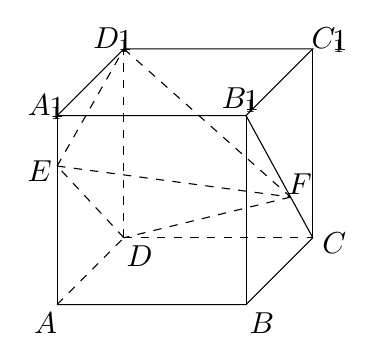
\begin{tikzpicture}[x=1bp,y=-1bp,
  every node/.style={inner sep=0,font=\fontsize{10.5pt}{12.6pt}\selectfont},
  line cap=butt, line join=miter]
  \draw[line width=0.398bp] (15.734,106.629) -- (83.746,106.629) -- (107.789,82.586);
  \draw[line width=0.398bp] (15.734,38.617) -- (83.746,38.617) -- (107.789,14.574) -- (39.777,14.574) -- (15.734,38.617);
  \draw[line width=0.398bp] (83.746,106.629) -- (83.746,38.617);
  \draw[line width=0.398bp] (107.785,82.586) -- (107.785,14.574);
  \draw[line width=0.398bp] (15.734,106.629) -- (15.734,38.617);
  \draw[line width=0.398bp] (83.746,38.617) -- (107.789,82.586);
  \draw[line width=0.398bp, dash pattern=on 2.989bp off 2.989bp] (15.734,106.629) -- (39.777,82.586);
  \draw[line width=0.398bp, dash pattern=on 2.989bp off 2.989bp] (39.777,82.586) -- (107.785,82.586);
  \draw[line width=0.398bp, dash pattern=on 2.989bp off 2.989bp] (39.777,82.586) -- (39.777,14.574);
  \draw[line width=0.398bp, dash pattern=on 2.989bp off 2.989bp] (39.777,82.586) -- (15.734,56.754);
  \draw[line width=0.398bp, dash pattern=on 2.989bp off 2.989bp] (15.734,56.754) -- (39.777,14.574);
  \draw[line width=0.398bp, dash pattern=on 2.989bp off 2.989bp] (39.777,14.574) -- (99.773,67.93);
  \draw[line width=0.398bp, dash pattern=on 2.989bp off 2.989bp] (99.773,67.93) -- (39.777,82.586);
  \draw[line width=0.398bp, dash pattern=on 2.989bp off 2.989bp] (15.734,56.754) -- (99.773,67.93);
  \node[anchor=base west] at (28.62,14.4) {$D_1$};
  \node[anchor=base west] at (37.31,15.29) {$1$};
  \node[anchor=base west] at (107.11,14.4) {$C_1$};
  \node[anchor=base west] at (114.62,15.29) {$1$};
  \node[anchor=base west] at (74.85,36.02) {$B_1$};
  \node[anchor=base west] at (82.82,36.91) {$1$};
  \node[anchor=base west] at (4.98,38.45) {$A_1$};
  \node[anchor=base west] at (12.85,39.35) {$1$};
  \node[anchor=base west] at (4.93,62.32) {$E$};
  \node[anchor=base west] at (98.72,67.05) {$F$};
  \node[anchor=base west] at (111.02,88.16) {$C$};
  \node[anchor=base west] at (40.57,93.09) {$D$};
  \node[anchor=base west] at (7.21,117.14) {$A$};
  \node[anchor=base west] at (84.8,117.14) {$B$};
\end{tikzpicture}
\end{center}
\nopagebreak[4]
\Needspace{4\baselineskip}
\textbf{解析}
三棱锥 $D_1-EDF$ 即 $F-ED_1D$。

\Needspace{5\baselineskip}
$\triangle ED_1D$ 在平面 $ADD_1A_1$ 内：底边 $DD_1=1$，$E$ 在棱 $AA_1$ 上，到直线 $DD_1$ 的距离等于 $AD=1$，故
\nopagebreak[4]
\[S_{\triangle ED_1D}=\frac12\times1\times1=\frac12.\]

\Needspace{5\baselineskip}
$F$ 在 $B_1C$ 上，而直线 $B_1C$ 平行于平面 $ADD_1A_1$，其上每一点到该平面的距离都等于棱长 $1$，故三棱锥的高为 $1$。于是
\nopagebreak[4]
\[V=\frac13\times\frac12\times1=\frac16.\]
（体积与 $E$，$F$ 在各自棱上的位置无关。）

\gkanswer{答案：$\dfrac16$。}

\end{answer}
\begin{answer}
\gksolhead{15}{}

\textbf{题目}：

设 $a>0$，若曲线 $y=\sqrt x$ 与直线 $x=a$，$y=0$ 所围成封闭图形的面积为 $a^2$，则 $a=$\gkblank{}。

\Needspace{4\baselineskip}
\textbf{解析}
\Needspace{5\baselineskip}
封闭图形由 $y=\sqrt x$，$x=a$，$y=0$ 围成，面积
\nopagebreak[4]
\[S=\int_0^a\sqrt x\,\mathrm dx=\frac23a^{\frac32}.\]
由 $\dfrac23a^{\frac32}=a^2$（$a>0$）得 $\sqrt a=\dfrac23$，故 $a=\dfrac49$。

\gkanswer{答案：$\dfrac49$。}

\end{answer}
\begin{answer}
\gksolhead{16}{}

\textbf{题目}：

如图，在平面直角坐标系 $xOy$ 中，一单位圆的圆心的初始位置在 $(0,1)$，此时圆上一点 $P$ 的位置在 $(0,0)$，圆在 $x$ 轴上沿正向滚动。当圆滚动到圆心位于 $(2,1)$ 时，$\overrightarrow{OP}$ 的坐标为\gkblank{}。
\nopagebreak[4]
\begin{center}%% ============================================================
%% f2012_shandong_sci_q16_rolling.tex
%% 2012 山东卷（理科）第 16 题 单位圆沿 x 轴正向滚动
%% 来源 PDF：普通高考/2012/2012山东理.pdf 第 1 页（印面 759）第 3 栏
%% 坐标取自原页矢量层（bp），原点为图区左上角 (890.0,262.0)，y 向下。
%% 第 266.6bp 处 31.4bp 的横线是题面填空横线，不属图稿，已排除。
%% ============================================================
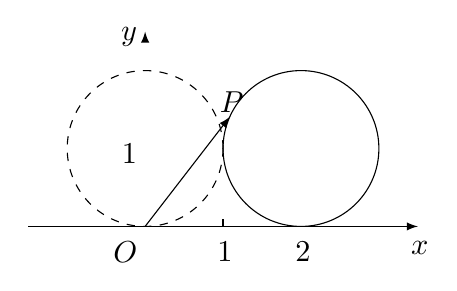
\begin{tikzpicture}[x=1bp,y=-1bp,
  every node/.style={inner sep=0,font=\fontsize{10.5pt}{12.6pt}\selectfont},
  line cap=butt, line join=miter]
  \draw[line width=0.398bp] (3.453,83.676) -- (140.133,83.676);
  \fill[black] (143.719,83.676) .. controls (142.656,83.477) and (140.93,82.879) .. (139.734,82.184) -- (139.734,85.168) .. controls (140.93,84.473) and (142.656,83.875) .. (143.719,83.676);
  \fill[black] (45.535,13.543) .. controls (45.336,14.605) and (44.738,16.332) .. (44.039,17.527) -- (47.027,17.527) .. controls (46.332,16.332) and (45.73,14.605) .. (45.535,13.543);
  \draw[line width=0.398bp] (73.586,83.676) -- (73.586,80.871);
  \draw[line width=0.398bp] (129.691,55.625) .. controls (129.691,40.129) and (117.133,27.57) .. (101.641,27.57) .. controls (86.145,27.57) and (73.586,40.129) .. (73.586,55.625) .. controls (73.586,71.117) and (86.145,83.676) .. (101.641,83.676) .. controls (117.133,83.676) and (129.691,71.117) .. (129.691,55.625) -- cycle;
  \draw[line width=0.398bp] (45.535,83.676) -- (73.816,47.055);
  \fill[black] (76.012,44.215) .. controls (75.203,44.934) and (73.672,45.938) .. (72.391,46.457) -- (74.758,48.285) .. controls (74.938,46.91) and (75.52,45.176) .. (76.012,44.215);
  \draw[line width=0.398bp, dash pattern=on 2.989bp off 2.989bp] (73.586,55.625) .. controls (73.586,40.129) and (61.027,27.57) .. (45.535,27.57) .. controls (30.039,27.57) and (17.48,40.129) .. (17.48,55.625) .. controls (17.48,71.117) and (30.039,83.676) .. (45.535,83.676) .. controls (61.027,83.676) and (73.586,71.117) .. (73.586,55.625) -- cycle;
  \node[anchor=base west] at (36.66,16.82) {$y$};
  \node[anchor=base west] at (72.28,42.56) {$P$};
  \node[anchor=base west] at (36.94,61.06) {$1$};
  \node[anchor=base west] at (141.11,93.96) {$x$};
  \node[anchor=base west] at (71.33,96.21) {$1$};
  \node[anchor=base west] at (99.39,96.21) {$2$};
  \node[anchor=base west] at (33.89,96.61) {$O$};
\end{tikzpicture}
\end{center}
\nopagebreak[4]
\Needspace{4\baselineskip}
\textbf{解析}
\Needspace{5\baselineskip}
圆的半径为 $1$，圆心由 $(0,1)$ 沿 $x$ 轴滚到 $(2,1)$，滚过的弧长为 $2$，故圆顺时针转过 $2$ 弧度。点 $P$ 初始在 $(0,0)$，即圆心正下方，相对圆心的坐标为 $(0,-1)$。顺时针旋转 $2$ 弧度后，相对圆心的坐标为
\nopagebreak[4]
\[(0\cdot\cos2+(-1)\sin2,\ -0\cdot\sin2+(-1)\cos2)=(-\sin2,\ -\cos2).\]
故 $P$ 的坐标为 $(2-\sin2,\ 1-\cos2)$。

\gkanswer{答案：$(2-\sin2,\ 1-\cos2)$。}

\end{answer}
\begin{answer}
\gksolhead{17}{}

\textbf{题目}：

已知向量 $\boldsymbol m=(\sin x,1)$，$\boldsymbol n=\left(\sqrt3A\cos x,\dfrac A2\cos2x\right)$（$A>0$），函数 $f(x)=\boldsymbol m\cdot\boldsymbol n$ 的最大值为 $6$。

（1） 求 $A$；

（2） 将函数 $y=f(x)$ 的图象向左平移 $\dfrac\pi{12}$ 个单位，再将所得图象上各点的横坐标缩短为原来的 $\dfrac12$ 倍，纵坐标不变，得到函数 $y=g(x)$ 的图象，求 $g(x)$ 在 $\left[0,\dfrac{5\pi}{24}\right]$ 上的值域。

\Needspace{4\baselineskip}
\textbf{解析}
\Needspace{5\baselineskip}
\textbf{（1）}
\nopagebreak[4]
\[f(x)=\boldsymbol m\cdot\boldsymbol n=\sqrt3A\sin x\cos x+\frac A2\cos2x=\frac{\sqrt3A}2\sin2x+\frac A2\cos2x=A\sin\left(2x+\frac\pi6\right).\]
由 $A>0$ 知 $f(x)$ 的最大值为 $A$，故 $A=6$。

\Needspace{5\baselineskip}
\textbf{（2）} 由（1）$f(x)=6\sin\left(2x+\dfrac\pi6\right)$。向左平移 $\dfrac\pi{12}$ 得
\nopagebreak[4]
\[y=6\sin\left(2\left(x+\frac\pi{12}\right)+\frac\pi6\right)=6\sin\left(2x+\frac\pi3\right).\]
\Needspace{5\baselineskip}
再将横坐标缩短为原来的 $\dfrac12$ 倍（即 $x$ 换成 $2x$），得
\nopagebreak[4]
\[g(x)=6\sin\left(4x+\frac\pi3\right).\]
当 $x\in\left[0,\dfrac{5\pi}{24}\right]$ 时，$4x+\dfrac\pi3\in\left[\dfrac\pi3,\dfrac{7\pi}6\right]$。在此区间上 $\sin$ 的最大值为 $1$（在 $4x+\dfrac\pi3=\dfrac\pi2$，即 $x=\dfrac\pi{24}$ 处取得），最小值为 $-\dfrac12$（在右端点 $\dfrac{7\pi}6$ 处取得）。故 $g(x)$ 的值域为 $[-3,6]$。

\gkanswer{答案（1）：$A=6$。}

\gkanswer{答案（2）：值域为 $[-3,6]$。}

\end{answer}
\begin{answer}
\gksolhead{18}{}

\textbf{题目}：

在如图所示的几何体中，四边形 $ABCD$ 是等腰梯形，$AB\parallel CD$，$\angle DAB=60^\circ$，$FC\perp$ 平面 $ABCD$，$AE\perp BD$，$CB=CD=CF$。

（1） 求证：$BD\perp$ 平面 $AED$；

（2） 求二面角 $F-BD-C$ 的余弦值。
\nopagebreak[4]
\begin{center}%% ============================================================
% f2012_shandong_sci_q18_solid.tex
%% 2012 山东卷（理科）第 18 题 几何体：等腰梯形 ABCD 为底，FC⊥平面 ABCD
%% 来源 PDF：普通高考/2012/2012山东理.pdf 第 2 页（印面 760）第 1 栏
%% 坐标取自原页矢量层（bp），原点为图区左上角 (240.0,138.0)，y 向下；虚线照原页。
%% ============================================================
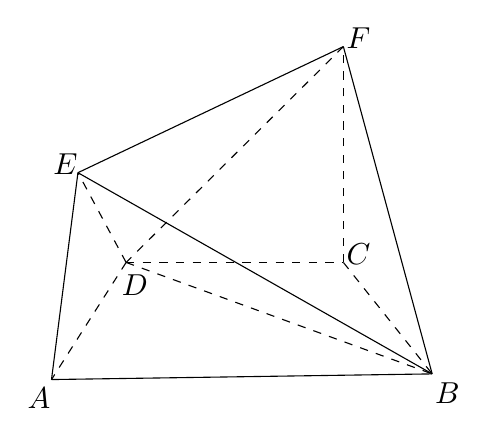
\begin{tikzpicture}[x=1bp,y=-1bp,
  every node/.style={inner sep=0,font=\fontsize{10.5pt}{12.6pt}\selectfont},
  line cap=butt, line join=miter]
  \draw[line width=0.3985bp] (24.035,50.133) -- (119.594,4.738);
  \draw[line width=0.3985bp] (24.035,50.133) -- (14.516,124.605);
  \draw[line width=0.3985bp] (151.559,122.566) -- (119.594,4.738);
  \draw[line width=0.3985bp] (151.559,122.566) -- (14.516,124.605);
  \draw[line width=0.3985bp] (24.035,50.133) -- (151.559,122.566);
  \draw[line width=0.3985bp, dash pattern=on 2.989bp off 2.989bp] (41.379,82.441) -- (24.035,50.133);
  \draw[line width=0.3985bp, dash pattern=on 2.989bp off 2.989bp] (41.379,82.441) -- (119.594,82.441);
  \draw[line width=0.3985bp, dash pattern=on 2.989bp off 2.989bp] (41.379,82.441) -- (14.516,124.605);
  \draw[line width=0.3985bp, dash pattern=on 2.989bp off 2.989bp] (41.379,82.441) -- (151.559,122.566);
  \draw[line width=0.3985bp, dash pattern=on 2.989bp off 2.989bp] (119.594,82.441) -- (119.594,4.738);
  \draw[line width=0.3985bp, dash pattern=on 2.989bp off 2.989bp] (119.594,4.738) -- (41.379,82.441);
  \draw[line width=0.3985bp, dash pattern=on 2.989bp off 2.989bp] (119.594,82.441) -- (151.559,122.566);
  \node[anchor=base west] at (120.56,5.38) {$F$};
  \node[anchor=base west] at (15.03,50.79) {$E$};
  \node[anchor=base west] at (120.53,83.11) {$C$};
  \node[anchor=base west] at (39.66,94.49) {$D$};
  \node[anchor=base west] at (152.39,133.12) {$B$};
  \node[anchor=base west] at (5.74,135.16) {$A$};
\end{tikzpicture}
\end{center}
\nopagebreak[4]
\Needspace{4\baselineskip}
\textbf{解析}
\textbf{（1）} 由等腰梯形 $AB\parallel CD$、$AD=BC$ 及 $\angle DAB=60^\circ$ 得 $\angle ADC=120^\circ$，$\angle C=120^\circ$。又 $CB=CD$。

\Needspace{5\baselineskip}
设 $CD=CB=AD=1$，则 $AB=CD+2AD\cos60^\circ=1+1=2$。在 $\triangle ABD$ 中
\nopagebreak[4]
\[BD^2=AB^2+AD^2-2AB\cdot AD\cos60^\circ=4+1-2=3,\]
故 $AD^2+BD^2=1+3=4=AB^2$，即 $\angle ADB=90^\circ$，$BD\perp AD$。

又 $AE\perp BD$ 且 $AD\cap AE=A$，所以 $BD\perp$ 平面 $AED$。

\Needspace{5\baselineskip}
\textbf{（2）} 以 $A$ 为原点，$AB$ 所在直线为 $x$ 轴建立空间直角坐标系。取 $CB=CD=CF=1$，则 $AB=2$，
\nopagebreak[4]
\[A(0,0,0),\quad B(2,0,0),\quad D\left(\frac12,\frac{\sqrt3}2,0\right),\quad C\left(\frac32,\frac{\sqrt3}2,0\right),\quad F\left(\frac32,\frac{\sqrt3}2,1\right).\]
平面 $CBD$ 即 $z=0$，法向量 $\boldsymbol n_1=(0,0,1)$。

\Needspace{5\baselineskip}
对平面 $FBD$：
\nopagebreak[4]
\[\overrightarrow{BD}=\left(-\frac32,\frac{\sqrt3}2,0\right),\qquad \overrightarrow{BF}=\left(-\frac12,\frac{\sqrt3}2,1\right),\]
\nopagebreak[4]
\[\boldsymbol n_2=\overrightarrow{BD}\times\overrightarrow{BF}=\left(\frac{\sqrt3}2,\ \frac32,\ -\frac{\sqrt3}2\right).\]

\Needspace{5\baselineskip}
设二面角 $F-BD-C$ 的大小为 $\theta$。由于 $\boldsymbol n_1$ 指向 $F$ 一侧的半空间、$\boldsymbol n_2$ 指向 $C$ 一侧，$\theta$ 与两法向量夹角互补，故
\nopagebreak[4]
\[\cos\theta=-\frac{\boldsymbol n_1\cdot\boldsymbol n_2}{|\boldsymbol n_1||\boldsymbol n_2|}=\frac{\frac{\sqrt3}2}{\sqrt{\frac34+\frac94+\frac34}\cdot1}=\frac{\frac{\sqrt3}2}{\sqrt{\frac{15}4}}=\frac{\sqrt5}5.\]
（也可直接用垂直于 $BD$ 的两条射线计算：$\overrightarrow{BF}$ 与 $\overrightarrow{BC}$ 在垂直于 $BD$ 方向上的分量分别为 $\left(\frac14,\frac{\sqrt3}4,1\right)$ 与 $\left(\frac14,\frac{\sqrt3}4,0\right)$，夹角余弦为 $\dfrac{\frac14}{\sqrt{\frac54}\cdot\frac12}=\dfrac{\sqrt5}5$。）

\gkanswer{答案（1）：证明见解析。}

\gkanswer{答案（2）：$\dfrac{\sqrt5}5$。}

\end{answer}
\begin{answer}
\gksolhead{19}{}

\textbf{题目}：

现有甲乙两个靶，某射手向甲靶射击一次命中的概率为 $\dfrac34$，命中得 $1$ 分，没有命中得 $0$ 分；向乙靶射击两次，每次命中的概率为 $\dfrac23$，每命中一次得 $2$ 分，没有命中得 $0$ 分。该射手每次射击的结果相互独立。假设该射手完成以上三次射击。

（1） 求该射手恰好命中一次的概率；

（2） 求该射手的总得分 $X$ 的分布列及数学期望 $EX$。

\Needspace{4\baselineskip}
\textbf{解析}
\textbf{（1）} 记「恰好命中一次」为事件 $E$。分两种互斥情形：
\begin{itemize}
\item 只命中甲靶：$\dfrac34\left(1-\dfrac23\right)^2=\dfrac34\cdot\dfrac19=\dfrac1{12}$；
\item 未命中甲靶、乙靶两次中恰命中一次：$\left(1-\dfrac34\right)\mathrm C_2^1\cdot\dfrac23\cdot\dfrac13=\dfrac14\cdot\dfrac49=\dfrac19$。
\end{itemize}

\Needspace{5\baselineskip}
故
\nopagebreak[4]
\[P(E)=\frac1{12}+\frac19=\frac7{36}.\]

\textbf{（2）} 设命中乙靶的次数为 $Y$，则 $Y\sim B\left(2,\dfrac23\right)$，且总得分 $X=2Y+\xi$，其中 $\xi$ 表示甲靶是否命中（命中为 $1$，否则为 $0$），$\xi$ 与 $Y$ 独立。

$Y$ 的分布：$P(Y=0)=\dfrac19$，$P(Y=1)=\dfrac49$，$P(Y=2)=\dfrac49$；$P(\xi=1)=\dfrac34$，$P(\xi=0)=\dfrac14$。

\Needspace{5\baselineskip}
于是 $X$ 的取值为 $0,1,2,3,4,5$：
\nopagebreak[4]
\[P(X=0)=\frac14\cdot\frac19=\frac1{36},\quad P(X=1)=\frac34\cdot\frac19=\frac1{12},\]
\nopagebreak[4]
\[P(X=2)=\frac14\cdot\frac49=\frac19,\quad P(X=3)=\frac34\cdot\frac49=\frac13,\]
\nopagebreak[4]
\[P(X=4)=\frac14\cdot\frac49=\frac19,\quad P(X=5)=\frac34\cdot\frac49=\frac13.\]
\Needspace{5\baselineskip}
（六个概率之和为 $1$，可作校验。）

\nopagebreak[4]
\[EX=E\xi+2EY=\frac34+2\times\frac43=\frac34+\frac83=\frac{41}{12}.\]

\gkanswer{答案（1）：$\dfrac7{36}$。}

\gkanswer{答案（2）：分布列 $P(X=0)=\dfrac1{36}$、$P(X=1)=\dfrac1{12}$、$P(X=2)=\dfrac19$、$P(X=3)=\dfrac13$、$P(X=4)=\dfrac19$、$P(X=5)=\dfrac13$；$EX=\dfrac{41}{12}$。}

\end{answer}
\begin{answer}
\gksolhead{20}{}

\textbf{题目}：

在等差数列 $\{a_n\}$ 中，$a_3+a_4+a_5=84$，$a_9=73$。

（1） 求数列 $\{a_n\}$ 的通项公式；

（2） 对任意 $m\in\mathbf N^*$，将数列 $\{a_n\}$ 中落入区间 $(9^m,9^{2m})$ 内的项的个数记为 $b_m$，求数列 $\{b_m\}$ 的前 $m$ 项和 $S_m$。

\Needspace{4\baselineskip}
\textbf{解析}
\Needspace{5\baselineskip}
\textbf{（1）} 设首项为 $a_1$，公差为 $d$。由 $a_3+a_4+a_5=3a_4=84$ 得 $a_4=28$。又 $a_9=73$，故
\nopagebreak[4]
\[d=\frac{a_9-a_4}{9-4}=\frac{45}5=9,\qquad a_1=a_4-3d=28-27=1.\]
\Needspace{5\baselineskip}
所以
\nopagebreak[4]
\[a_n=1+9(n-1)=9n-8.\]

\Needspace{5\baselineskip}
\textbf{（2）} 由 $9^m<9n-8<9^{2m}$ 得
\nopagebreak[4]
\[\frac{9^m+8}9<n<\frac{9^{2m}+8}9,\]
\Needspace{5\baselineskip}
即 $9^{m-1}+\dfrac89<n<9^{2m-1}+\dfrac89$。由于 $n$ 为整数，
\nopagebreak[4]
\[9^{m-1}+1\leqslant n\leqslant9^{2m-1},\]
\Needspace{5\baselineskip}
故
\nopagebreak[4]
\[b_m=9^{2m-1}-9^{m-1}.\]
\Needspace{5\baselineskip}
于是
\nopagebreak[4]
\[S_m=\sum_{k=1}^m\left(9^{2k-1}-9^{k-1}\right)=9\cdot\frac{81^m-1}{80}-\frac{9^m-1}8=\frac{9\cdot81^m-10\cdot9^m+1}{80}.\]

\gkanswer{答案（1）：$a_n=9n-8$。}

\gkanswer{答案（2）：$S_m=\dfrac{9\cdot81^m-10\cdot9^m+1}{80}$。}

\end{answer}
\begin{answer}
\gksolhead{21}{}

\textbf{题目}：

在平面直角坐标系 $xOy$ 中，$F$ 是抛物线 $C:x^2=2py$（$p>0$）的焦点，$M$ 是抛物线 $C$ 上位于第一象限内的任意一点，过 $M$，$F$，$O$ 三点的圆的圆心为 $Q$，点 $Q$ 到抛物线 $C$ 的准线的距离为 $\dfrac34$。

（1） 求抛物线 $C$ 的方程；

（2） 是否存在点 $M$，使得直线 $MQ$ 与抛物线 $C$ 相切于点 $M$？若存在，求出点 $M$ 的坐标；若不存在，说明理由；

（3） 若点 $M$ 的横坐标为 $\sqrt2$，直线 $l:y=kx+\dfrac14$ 与抛物线 $C$ 有两个不同的交点 $A$，$B$，$l$ 与圆 $Q$ 有两个不同的交点 $D$，$E$，求当 $\dfrac12\leqslant k\leqslant2$ 时，$|AB|^2+|DE|^2$ 的最小值。

\Needspace{4\baselineskip}
\textbf{解析}
\Needspace{5\baselineskip}
\textbf{（1）} 抛物线 $x^2=2py$ 的焦点 $F\left(0,\dfrac p2\right)$，准线 $y=-\dfrac p2$。圆心 $Q$ 到 $O$ 与 $F$ 等距，故 $Q$ 在 $OF$ 的垂直平分线 $y=\dfrac p4$ 上。设 $Q\left(x_Q,\dfrac p4\right)$，则 $Q$ 到准线的距离为
\nopagebreak[4]
\[\frac p4+\frac p2=\frac{3p}4=\frac34,\]
故 $p=1$，抛物线 $C$ 的方程为 $x^2=2y$。

\Needspace{5\baselineskip}
\textbf{（2）} 设 $M\left(x_0,\dfrac{x_0^2}2\right)$（$x_0>0$）。$C$ 在 $M$ 处的切线斜率为 $x_0$，切线方程为
\nopagebreak[4]
\[y-\frac{x_0^2}2=x_0(x-x_0),\quad\text{\text{即}}\quad y=x_0x-\frac{x_0^2}2.\]
\Needspace{5\baselineskip}
若 $Q$ 在切线上，由 $y_Q=\dfrac14$ 得
\nopagebreak[4]
\[x_Q=\frac{\frac14+\frac{x_0^2}2}{x_0}.\]
\Needspace{5\baselineskip}
又 $|QO|=|QM|$，即 $2\overrightarrow{OQ}\cdot\overrightarrow{OM}=|OM|^2$，亦即
\nopagebreak[4]
\[2\left(x_Qx_0+\frac{x_0^2}8\right)=x_0^2+\frac{x_0^4}4\quad\Rightarrow\quad x_Q=\frac{3x_0+x_0^3}8.\]
\Needspace{5\baselineskip}
两式联立得
\nopagebreak[4]
\[\frac{\frac14+\frac{x_0^2}2}{x_0}=\frac{3x_0+x_0^3}8\ \Rightarrow\ x_0^4-x_0^2-2=0,\]
\Needspace{5\baselineskip}
故 $x_0^2=2$，$x_0=\sqrt2$（第一象限）。所以存在这样的点
\nopagebreak[4]
\[M(\sqrt2,1).\]

\Needspace{5\baselineskip}
\textbf{（3）} 由（2）$M(\sqrt2,1)$，此时 $x_Q=\dfrac{3\sqrt2+2\sqrt2}8=\dfrac{5\sqrt2}8$，即
\nopagebreak[4]
\[Q\left(\frac{5\sqrt2}8,\frac14\right),\qquad R^2=|QO|^2=\frac{25}{32}+\frac1{16}=\frac{27}{32}.\]

\Needspace{5\baselineskip}
直线 $l:y=kx+\dfrac14$ 与 $x^2=2y$ 联立得
\nopagebreak[4]
\[x^2-2kx-\frac12=0,\]
\Needspace{5\baselineskip}
故 $x_A+x_B=2k$，$x_Ax_B=-\dfrac12$，从而
\nopagebreak[4]
\[|AB|^2=(1+k^2)\left[(x_A+x_B)^2-4x_Ax_B\right]=(1+k^2)(4k^2+2).\]

\Needspace{5\baselineskip}
$Q$ 到 $l$ 的距离
\nopagebreak[4]
\[d=\frac{\left|k\cdot\frac{5\sqrt2}8-\frac14+\frac14\right|}{\sqrt{1+k^2}}=\frac{5\sqrt2\,k}{8\sqrt{1+k^2}},\]
\Needspace{5\baselineskip}
故
\nopagebreak[4]
\[|DE|^2=4(R^2-d^2)=\frac{27}8-\frac{25k^2}{8(1+k^2)}.\]

\Needspace{5\baselineskip}
于是
\nopagebreak[4]
\[|AB|^2+|DE|^2=(1+k^2)(4k^2+2)+\frac{27}8-\frac{25k^2}{8(1+k^2)}.\]
\Needspace{5\baselineskip}
令 $t=k^2\in\left[\dfrac14,4\right]$，
\nopagebreak[4]
\[F(t)=4t^2+6t+\frac{35}8-\frac{25t}{8(1+t)}.\]
\Needspace{5\baselineskip}
其导函数
\nopagebreak[4]
\[F'(t)=8t+6-\frac{25}{8(1+t)^2},\]
且 $F''(t)=8+\dfrac{25}{4(1+t)^3}>0$，故 $F'$ 递增；又 $F'\left(\dfrac14\right)=6>0$，所以 $F'(t)>0$ 在 $\left[\dfrac14,4\right]$ 上成立。
\Needspace{5\baselineskip}
故 $F$ 在 $\left[\dfrac14,4\right]$ 上单调递增，当 $t=\dfrac14$（即 $k=\dfrac12$）时取最小值
\nopagebreak[4]
\[F\left(\frac14\right)=\frac{13}2.\]

\gkanswer{答案（1）：$x^2=2y$。}

\gkanswer{答案（2）：存在，$M(\sqrt2,1)$。}

\gkanswer{答案（3）：最小值为 $\dfrac{13}2$。}

\end{answer}
\begin{answer}
\gksolhead{22}{}

\textbf{题目}：

已知函数 $f(x)=\dfrac{\ln x+k}{\mathrm e^x}$（$k$ 为常数，$\mathrm e=2.71828\cdots$ 是自然对数的底数），曲线 $y=f(x)$ 在点 $(1,f(1))$ 处的切线与 $x$ 轴平行。

（1） 求 $k$ 的值；

（2） 求 $f(x)$ 的单调区间；

（3） 设 $g(x)=(x^2+x)f'(x)$，其中 $f'(x)$ 为 $f(x)$ 的导函数。证明：对任意 $x>0$，$g(x)<1+\mathrm e^{-2}$。

\Needspace{4\baselineskip}
\textbf{解析}
\Needspace{5\baselineskip}
\textbf{（1）}
\nopagebreak[4]
\[f'(x)=\frac{\frac1x-\ln x-k}{\mathrm e^x}.\]
由 $f'(1)=0$ 得 $1-k=0$，故 $k=1$。

\textbf{（2）} 此时 $f'(x)=\dfrac{\frac1x-\ln x-1}{\mathrm e^x}$。令 $h(x)=\dfrac1x-\ln x-1$，则 $h'(x)=-\dfrac1{x^2}-\dfrac1x<0$，$h$ 在 $(0,+\infty)$ 上递减，且 $h(1)=0$。故 $0<x<1$ 时 $f'(x)>0$，$x>1$ 时 $f'(x)<0$，即 $f$ 在 $(0,1)$ 上递增，在 $(1,+\infty)$ 上递减。

\Needspace{5\baselineskip}
\textbf{（3）} 由（1）$f'(x)=\dfrac{\frac1x-\ln x-1}{\mathrm e^x}$，故
\nopagebreak[4]
\[g(x)=(x^2+x)f'(x)=\frac{(x+1)\left(1-x-x\ln x\right)}{\mathrm e^x}.\]
\Needspace{5\baselineskip}
记 $\varphi(x)=1-x-x\ln x$。由 $\varphi'(x)=-2-\ln x$ 知 $\varphi$ 在 $\left(0,\mathrm e^{-2}\right)$ 上递增、在 $\left(\mathrm e^{-2},+\infty\right)$ 上递减，最大值为
\nopagebreak[4]
\[\varphi\left(\mathrm e^{-2}\right)=1-\mathrm e^{-2}+2\mathrm e^{-2}=1+\mathrm e^{-2}.\]
又 $\dfrac{x+1}{\mathrm e^x}$ 在 $(0,+\infty)$ 上递减（其导数为 $-\dfrac{x}{\mathrm e^x}<0$）。

\begin{itemize}
\item 当 $0<x\leqslant\mathrm e^{-2}$ 时，$\dfrac{x+1}{\mathrm e^x}<1$，故
\end{itemize}
\nopagebreak[4]
\[g(x)<\varphi(x)\leqslant1+\mathrm e^{-2}.\]
\begin{itemize}
\item 当 $x>\mathrm e^{-2}$ 时，$\dfrac{x+1}{\mathrm e^x}\leqslant\dfrac{1+\mathrm e^{-2}}{\mathrm e^{\mathrm e^{-2}}}$，故
\end{itemize}
\nopagebreak[4]
\[g(x)\leqslant\left(1+\mathrm e^{-2}\right)\cdot\frac{1+\mathrm e^{-2}}{\mathrm e^{\mathrm e^{-2}}}.\]
\Needspace{5\baselineskip}
由 $\ln\left(1+\mathrm e^{-2}\right)<\mathrm e^{-2}$ 得 $1+\mathrm e^{-2}<\mathrm e^{\mathrm e^{-2}}$，故
\nopagebreak[4]
\[\frac{\left(1+\mathrm e^{-2}\right)^2}{\mathrm e^{\mathrm e^{-2}}}<1+\mathrm e^{-2},\]
即此时也有 $g(x)<1+\mathrm e^{-2}$。

综上，对任意 $x>0$，$g(x)<1+\mathrm e^{-2}$。

\gkanswer{答案（1）：$k=1$。}

\gkanswer{答案（2）：递增区间 $(0,1)$，递减区间 $(1,+\infty)$。}

\gkanswer{答案（3）：证明见解析。}

\end{answer}